\documentclass[11pt]{article}

\usepackage{graphicx}
\usepackage[margin=1in]{geometry}
\usepackage[dvipsnames]{xcolor}
\usepackage[most]{tcolorbox}
\usepackage[colorlinks=true, linkcolor=blue]{hyperref}
\usepackage{subcaption, float}
\usepackage{tabularray, booktabs}
\usepackage{listings}
\UseTblrLibrary{booktabs}

\newtcolorbox{definition}[1][]{
  colback=blue!5!white,
  colframe=blue!75!black,
  fonttitle=\bfseries,
  title=Definition: #1
}

\newtcolorbox{warning}[1][]{
  colback=red!5!white,
  colframe=red!75!black,
  fonttitle=\bfseries,
  title=#1
}

\newtcolorbox{note}[1][]{
  colback=green!5!white,
  colframe=green!75!black,
  fonttitle=\bfseries,
  title=#1,
  breakable
}

\newtcolorbox{note_special}[1][]{
  colback=orange!5!white,
  colframe=orange!75!black,
  fonttitle=\bfseries,
  title=#1,
  breakable
}

\definecolor{codegreen}{rgb}{0,0.6,0}
\definecolor{codegray}{rgb}{0.5,0.5,0.5}
\definecolor{codepurple}{rgb}{0.58,0,0.82}
\definecolor{backcolour}{rgb}{0.95,0.95,0.92}

\lstdefinestyle{mystyle}{
    backgroundcolor=\color{backcolour},   
    commentstyle=\color{codegreen},
    keywordstyle=\color{magenta},
    numberstyle=\tiny\color{codegray},
    stringstyle=\color{codepurple},
    basicstyle=\ttfamily\footnotesize,
    breakatwhitespace=false,         
    breaklines=true,                 
    captionpos=b,                    
    keepspaces=true,                 
    % numbers=left,                    
    numbersep=5pt,                  
    showspaces=false,                
    showstringspaces=false,
    showtabs=false,                  
    tabsize=2
}

\lstset{style=mystyle}

\begin{document}

\begin{titlepage}
    \centering
    
    
\includegraphics[width=0.4\textwidth]{UCT-logo.png}\\[2cm] 
    
    \textsc{\LARGE University of Cape Town}\\[1.5cm]
    
    \rule{\linewidth}{0.5mm} \\[0.4cm]
    { \huge \bfseries CSC2042S: Machine Learning \\[0.4cm] }
    \rule{\linewidth}{0.5mm} \\[1.5cm]
    
    { \Large Author: George Goodey }
    
    \vfill

    {\large \today}
    
\end{titlepage}

\tableofcontents
\newpage

\section{Supervised learning}

\subsection{What is machine learning?}
\begin{definition}[Machine Learning]
Machine learning is the study of algorithms that:
\begin{itemize}
    \item improve their performance $P$ (according to a criterion that measures success)
    \item at some task $T$
    \item with experience $E$ (from data examples).
\end{itemize}
\end{definition}
$\quad$\\[0em]
A well-defined task is given by $<P,T,E>$. For example:
\begin{itemize}
    \item \textbf{Image classification:} $<$Accuracy, Classify handwritten digits, Dataset of labelled images$>$.
    \item \textbf{Chess:} $<$Playing quality, Play chess against human, Dataset of old games$>$.
    \item \textbf{ChatGPT:} $<$Quality of conversation, Generate responses, All text on the web$>$.
\end{itemize}

\subsection{Types of machine learning}
There are many types:
\begin{itemize}
    \item Supervised learning.
    \item Unsupervised learning.
    \item Reinforcement learning.
    \item etc.
\end{itemize}

\subsubsection{Unsupervised learning}
The problem is framed as finding structure in $x$ without labels (no $y$). Inputs are examples in the dataset represented by \textit{features}. Data $D$ is $|D|$ examples $\{x_1,x_2,\dots,x_{|D|}\}$ without any labels. Given a new example $x$, where does this fit into the data? 
For a more detailed overview of unsupervised learning, please look at the later section.

\subsubsection{Supervised learning}
The problem is framed as mapping inputs $x$ to outputs $y$. Inputs are examples in the dataset represented by \textit{features}. and outputs are \textit{labels} describing the data examples.
Data $D$ is $|D|$ pairs $\{(x_1,y_1),(x_2,y_2),\dots,(x_{|D|},y_{|D|})\}$. The goal of supervised learning is to learn a function $h:X\to Y$ that can map inputs to outputs. Given a new example $x$, you can use $h(x)$ to predict the output.
\begin{figure}[H]
    \centering
    \begin{subfigure}{0.7\textwidth}
        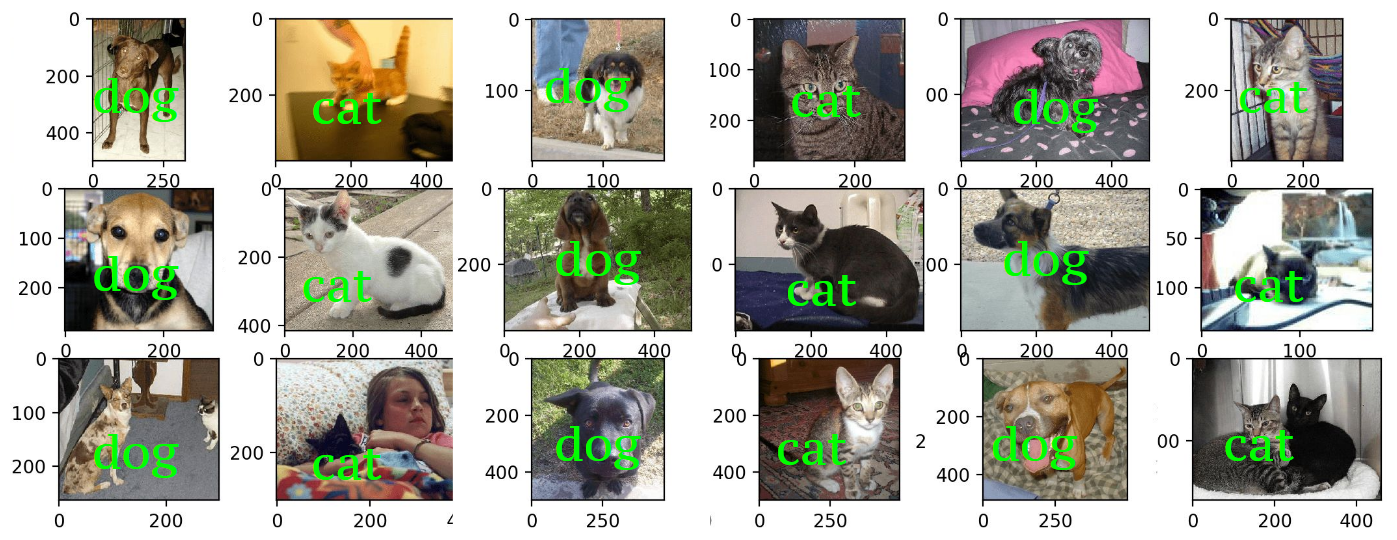
\includegraphics[width=\linewidth]{Pictures/supervised_1.png}
    \end{subfigure}
\end{figure}

\subsection{Types of supervised learning}
The two different types are distinguished by the type of the tagret variable $y$:
\begin{itemize}
    \item \textbf{Classification:} Predict a \textbf{discrete/categorical} target variable i.e. from a set of possible values.
    \item \textbf{Regression:} Predict a \textbf{continuous} target variable i.e. output can be any real valued number in a range.
\end{itemize}
\begin{figure}[H]
    \centering
    \begin{subfigure}{0.7\textwidth}
        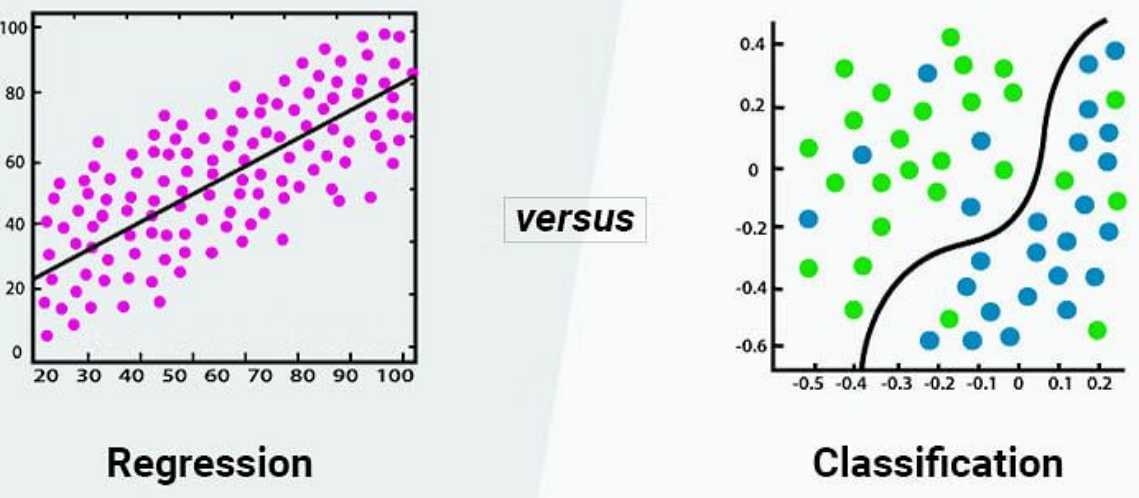
\includegraphics[width=\linewidth]{Pictures/supervised_2.png}
    \end{subfigure}
\end{figure}

\subsection{What is a machine learning model?}
\begin{figure}[H]
    \centering
    \begin{subfigure}{0.7\textwidth}
        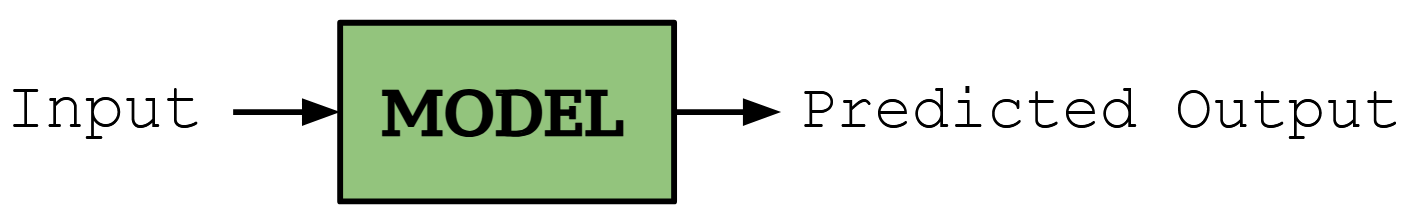
\includegraphics[width=\linewidth]{Pictures/supervised_3.png}
    \end{subfigure}
\end{figure}
\begin{definition}[Model]
A \textbf{model} is a mathematical representation of a real-world process used to make predictions or decisions. A model is defined by its:
\begin{itemize}
    \item \textbf{architecture}, the type of machine learning model (e.g perceptron, logistic regression, a neural network)
    \item and its \textbf{parameters}, the internal components (numerical values) of the model that are leanred from datt to accurately represent the data.
\end{itemize}
\end{definition}

\subsection{Terminology}
\begin{definition}[Training]
\textbf{Training} is the process of teaching a machine learning model to make predictions or decisions based on data. The model learns patterns and relationships from a dataset to improve its performance.
\begin{figure}[H]
    \centering
    \begin{subfigure}{0.7\textwidth}
        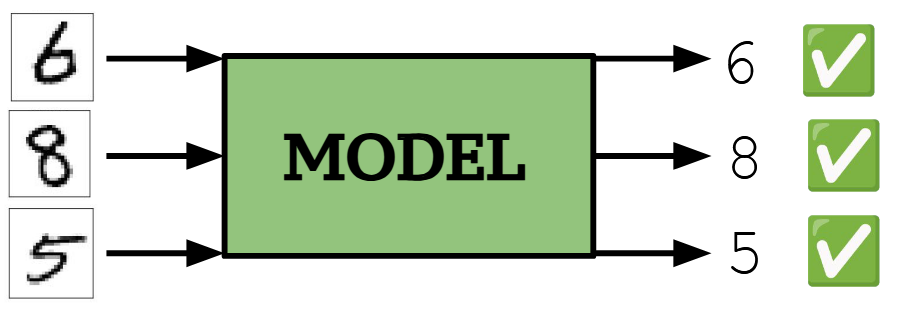
\includegraphics[width=\linewidth]{Pictures/supervised_4.png}
    \end{subfigure}
\end{figure}
\end{definition}
\begin{definition}[Parameter]
A \textbf{parameter} is a variable in a model that the algorithm adjusts during training. Parameters are the internal components of the model that are learned from the data to make accurate predictions.
\end{definition}
\subsubsection{Linear regression example}
We want to predict the house price for an estate agent. Given the number of rooms $x$ in a house, what price $y$ should it sell for?
\\\\
We can use a simple formula:
\begin{figure}[H]
    \centering
    \begin{subfigure}{0.7\textwidth}
        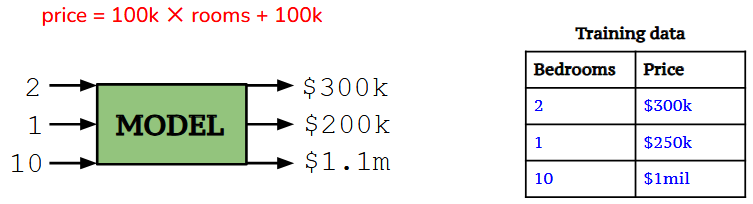
\includegraphics[width=\linewidth]{Pictures/supervised_5.png}
    \end{subfigure}
\end{figure}
$\quad$\\[-1em]
This is called a linear regression model and can be formalized as: 
Let $x$ be the number of rooms and $y$ be the predicted price, then $y=wx+b$.
The parameters $w$ and $b$ are values we want to learn during training.

\subsection{Perceptron}
\begin{definition}[Perceptron]
The perceptron is a binary classifier. For a given input vector $x$, it predicts one of two classes as output (represented by 0 or 1) with a step function.
\end{definition}
\begin{figure}[H]
    \centering
    \begin{subfigure}{0.4\textwidth}
        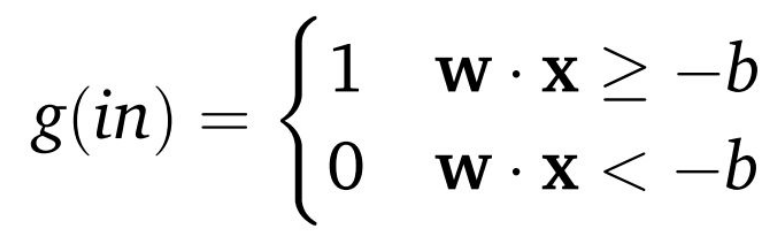
\includegraphics[width=\linewidth]{Pictures/perceptron_1.png}
    \end{subfigure}
\end{figure}
$\quad$\\[-1em]
The input $x$ is passed through a weighted sum, the result of which is passed through the step function.
\begin{itemize}
    \item $\mathbf{x}$ is the input vector,
    \item $\mathbf{w}$ is the weight vector, and
    \item $b$ is the bias term.
\end{itemize}
The perceptron is a linear, binary classification algorithm. It is \textbf{binary} since we classify input into one of two classes e.g. negative or positive.
It is also \textbf{linear} because the classification decision is based on a value that is a linear combination of input values $(x_1,x_2,\dots,x_n)$.
\begin{figure}[H]
    \centering
    \begin{subfigure}{0.6\textwidth}
        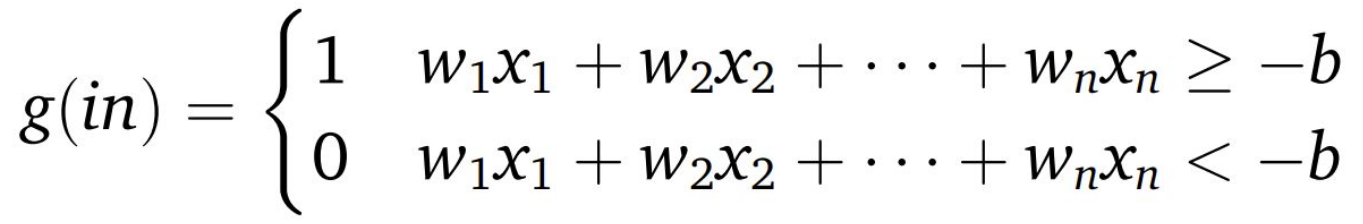
\includegraphics[width=\linewidth]{Pictures/perceptron_2.png}
    \end{subfigure}
\end{figure}
$\quad$\\[-1em]
What can we do with perceptrons? We can implement primitive boolean functions!
\begin{figure}[H]
    \centering
    \begin{subfigure}{0.7\textwidth}
        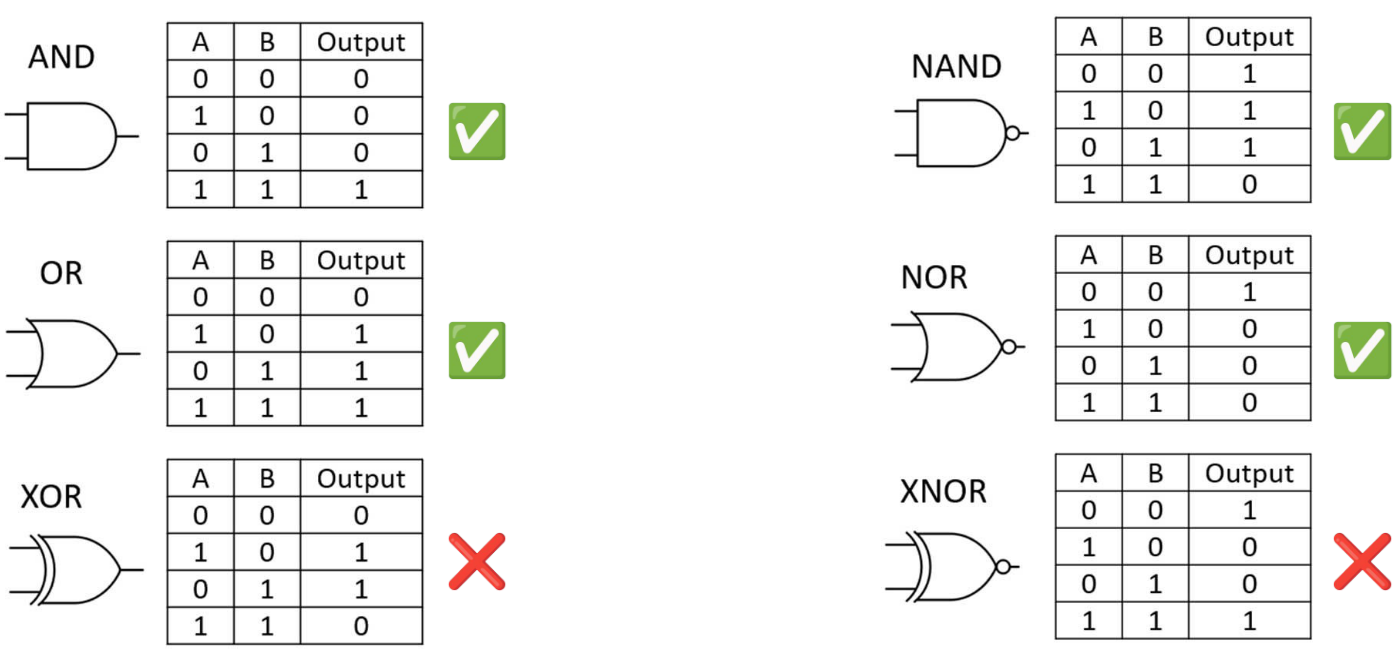
\includegraphics[width=\linewidth]{Pictures/perceptron_3.png}
    \end{subfigure}
\end{figure}

\subsection{Perceptron learning rule}
\begin{definition}[Optimization]
\textbf{Optimization} is the mathematical process of finding the best parameters for machine learning model for a specific task.
\end{definition}
$\quad$\\[-1em]
We considering a binary (0 or 1) classification problem. Can we find the weights and bias that would classify inputs $x$ correctly as either 0 or 1?
\begin{figure}[H]
    \centering
    \begin{subfigure}{0.7\textwidth}
        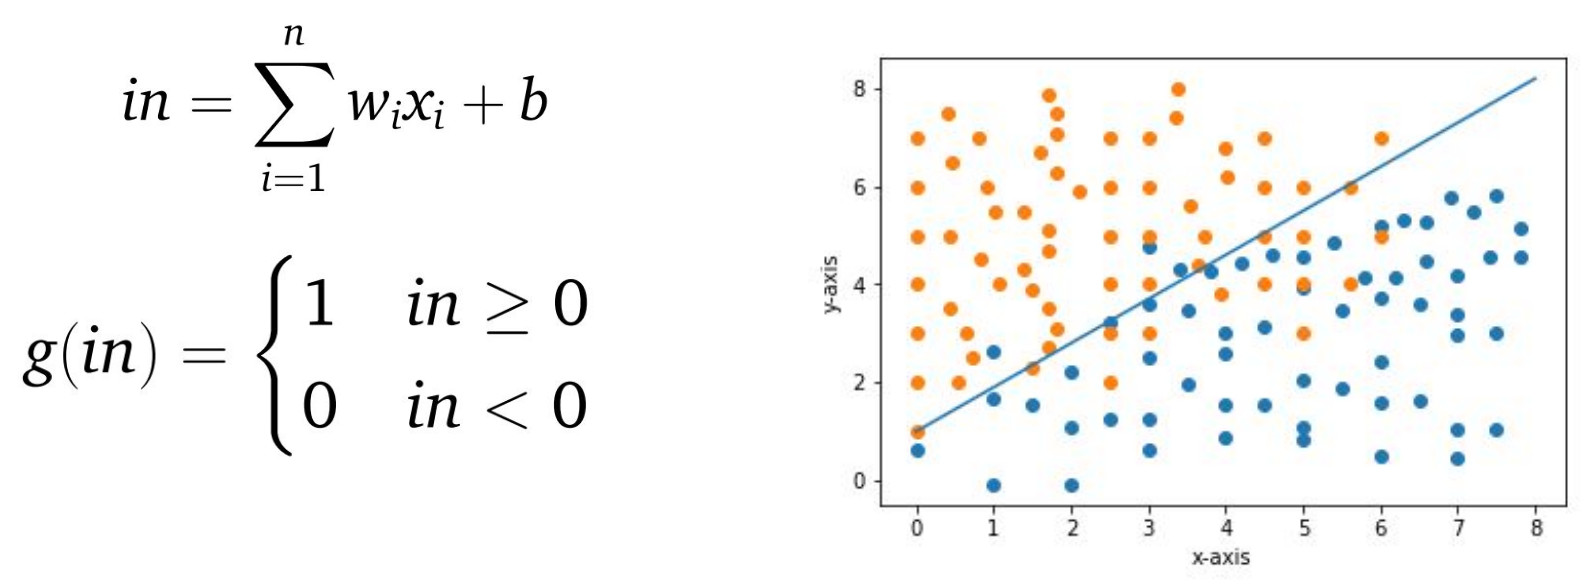
\includegraphics[width=\linewidth]{Pictures/perceptron_4.png}
    \end{subfigure}
\end{figure}
$\quad$\\[-1em]
There is a simple weight update rule that converges to a solution that classifies data perfectly (if the data is linearly separable).
For a single data example $(\mathbf{x},y)$, where $\mathbf{x}$ is a vector:
\begin{align*}
    \mathbf{w}&\leftarrow\mathbf{w}+\alpha(y-g(\mathbf{x}))\mathbf{x} \\
    b&\leftarrow b+\alpha(y-g(\mathbf{x}))
\end{align*}
$\alpha$, which is always positive, is called the \textbf{learning rate} (size of parameter updates).
We specify this ourselves. It is an example of a hyperparameter. If it's too big, the model might not converge.
If it's too small, the model might take too long to converge.
\begin{definition}[Hyperparameter]
A \textbf{hyperparameter} is a configuration variable external to the model whose value is fixed before training begins. Hyperparameters control the learning process and the structure of the model.
\end{definition}
\subsubsection{Error correction learning algorithm}
\begin{enumerate}
    \item Initialize all weights randomly.
    \item For each training example, apply the perceptron learning rule.
    \item Repeat untill the error is acceptable or $N$ iterations (cutoff) is reached.
\end{enumerate}
\subsubsection{Train/validation/test sets}
Datasets are usually split into 3 subsets.
\begin{itemize}
    \item \textbf{Training set:} data used to train your machine learning model (the learning process).
    \item \textbf{Validation set:} data used to evaluate model performance during
    \begin{itemize}
        \item Training: track performance while model is learning.
        \item Development: compare modelling decisions and configurations e.g. hyperparameter settings.
    \end{itemize}
    \item \textbf{Test set:} data used to evaluate performance once the final model has been trained e.g. compare perceptron to other types of models.
\end{itemize}
Datasets are used in two ways:
\begin{itemize}
    \item Training sets are used for learning: update model parameters based on data in the training set.
    \item Validation and test sets are used for evaluation. You only use it for prediction, comparing model outputs to expected outputs or evaluate model performance on data that it was not trained on.
\end{itemize}
\begin{warning}[Super important]
Do not train your model on your validation or test sets!
\end{warning}
$\quad$\\[-1em]
Usually, the full dataset is split into train/validation/test sets proportionally e.g. 80\%/10\%/10\%.
You want to train on most of the data (maximize performance). You want to test your model on data that it hasn't seen before. Why?
To evaluate if your model is generalizing to new examples. If you test your model on data which it was trained, maybe it's just memorizing specific training examples.
\begin{definition}[Data leakage]
\textbf{Data leakage} is when test data is "contaminated" with training data, so we are not getting a reliable evaluation of performance.
\end{definition}
\subsubsection{Training loop}
\begin{definition}[Training loop]
A \textbf{training loop} is the process of going through the whole training set once which is called an \textbf{epoch} of training. Training takes time, potentially requires multiple epochs.
\end{definition}
$\quad$\\[-1em]
We need to go through the entire training set, on example at a time, each time updating parameters with the perceptron learning rule. 
Train for multiple epochs, logging validation accuracy at regular intervals to track performance e.g. after each epoch or after every $M$ parameter updates, where $M$ is fixed and specified by the programmer.
\begin{lstlisting}[language=Python]
Create new perceptron P with randomly initialized weights and bias for number of epochs E:

    # Learn from the training data
    for each example (x_i, y_i) in the training set:
        P.apply_learning_rule(x_i, y_i)
    
    # Evaluate on the validation data
    for each example (x_i, y_i) in the validation set:
        P.predict(x_i, y_i) and store prediction
    
    Print the current validation accuracy
\end{lstlisting}
During development, you should try different hyperparameter settings. For a perceptron, train models with different learning rates.
\subsubsection{Perceptron convergence}
\begin{definition}[Convergence]
\textbf{Convergence} is when the algorithm finds weights and bias such that all training examples are classified correctly, after which $\mathbf{w}$ and $b$ reamin unchanged.
\end{definition}
$\quad$\\[-1em]
The perceptron learning algorithm is guaranteed to converge to a solution in finite steps if:
\begin{itemize}
    \item training examples are linearly separable, and
    \item learning rate is sufficiently small.
\end{itemize}
\begin{warning}[Important]
If the data is not linearly separable, the algorithm never converges. It will keeps updating parameters indefinitely!
\end{warning}
$\quad$\\[-1em]
Handling linearly non-separable data:
\begin{itemize}
    \item In practice, we often apply the perceptron even when data is not perfectly separable.
    \item Perceptrons can still learn a "good enough" separator that minimizes errors, though not perfect.
    \item To avoid endless updates, we must define stopping conditions that ensure that algorithm halts, even if perfect classification is impossible.
\end{itemize}
Potential stopping criteria:
\begin{itemize}
    \item \textbf{Maximum number of epochs:} stop training after a fixed number $E$ of full passes through the training set.
    \item \textbf{Maximum number of updates:} stop training after a fixed number $M$ of perceptron learning rule applications.
    \item \textbf{Early stopping:} stop when the validation accuracy stops improving for a predetermined number of training epochs $P$ or training steps $S$.
\end{itemize}

\subsection{Multi-class classification}
The problem is framed as mapping inputs $x$ to outputs $y$, where $y\in\{1,\dots, K\}$ with $K>2$. The target variable is still discrete and can only take a finite set of possible values, which are knwown in advance.
Many taks can be framed in this way:
\begin{itemize}
    \item \textbf{News categorization:} predict if an article is sport/politics/tech.
    \item \textbf{Mood prediction:} categorize customer feedback as happy/sad/angry/neutral.
    \item \textbf{Face identification:} determine which of your 100+ instagram friends are in a photo.
\end{itemize}
\subsubsection{One-vs-rest classification}
A way to use binary classification models for multi-class classification.
\begin{itemize}
    \item Train $K$ binary classifiers.
    \item Each classifier is trained to classify one class against all other classes.
    \item To make a prediction for a data point, all $K$ classifiers are used. The class predicted with the largest margin is taken as the predicted class.
\end{itemize}
For $K$-class classification, train $K$ perceptrons:
$$
g_c(\mathbf{x})=\begin{cases}
    1 & \mathbf{w}_c\cdot \mathbf{x}+b_c\ge 0 \\
    0 & \mathbf{w}_c\cdot \mathbf{x}+b_c < 0
\end{cases}
\quad\quad
\text{for each class }c\in\{0,\dots,K-1\}
$$
Each perceptron has its own weight vector $\mathbf{w}_c$ and bias $b_c$. But the final multi-class prediction is not this binary output- it's based on the weighted sum $\mathbf{w}_c\cdot\mathbf{x}+b_c$, which is the "score" given for class $c$.
To make a final decision, we compute all the linear scores:
$$
s_c(\mathbf{x})=\mathbf{w}_c\cdot\mathbf{x}+b_c\quad\quad\text{for each class }c\in\{1,\dots,K-1\}
$$
and then choose the predicted class as the one with the largest score:
$$
\hat{y}=\underset{c\in\{0,\dots,K-1\}}{\text{argmax}}s_c(\mathbf{x})
$$
where $\hat{y}$ is the prediction. Each perceptron predicts "is this class $c$ or not?" The one-vs-rest multi-class perceptron chooses the class whose perceptron is most confident.
\subsubsection{Evaluation metrics}
$$
\text{accuracy}=\frac{\text{\# correct predictions }(\hat{y}=y)}{\text{\# total predictions (evaluation dataset size)}}
$$
The accuracy is a single number to summarize and compare classifier performance. But it can also be skewed in some cases e.g. when one class occurs a lot more than others.
$$
\text{error}=1-\text{accuracy}
$$
In some tasks, we care more about one class (e.g. rare positive cases). Sometimes the priority is to detect all positives, even if that means more false alarms e.g. disease diagnosis, fraud detection.
Other times the priority is to avoid false positives, even if that means missing some positives, e.g. spam filters.
\begin{figure}[H]
    \centering
    \begin{subfigure}{0.49\textwidth}
        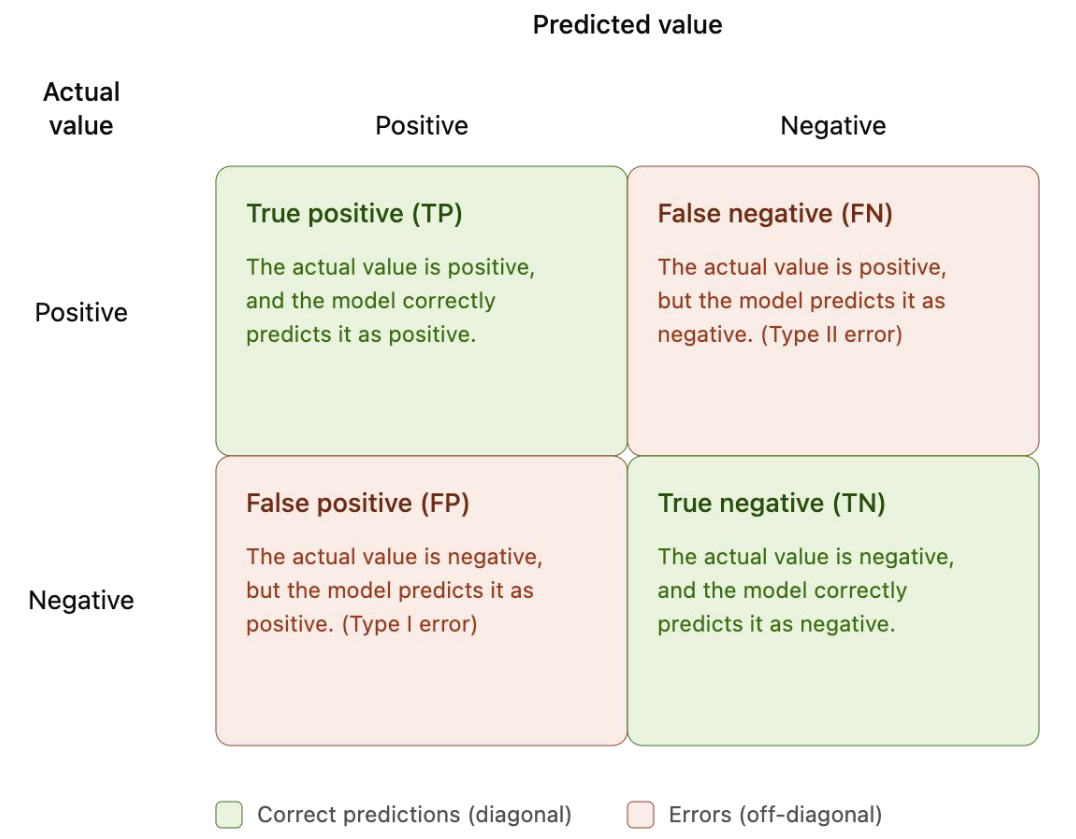
\includegraphics[width=\linewidth]{Pictures/multiclass_1.png}
    \end{subfigure}
    \begin{subfigure}{0.49\textwidth}
        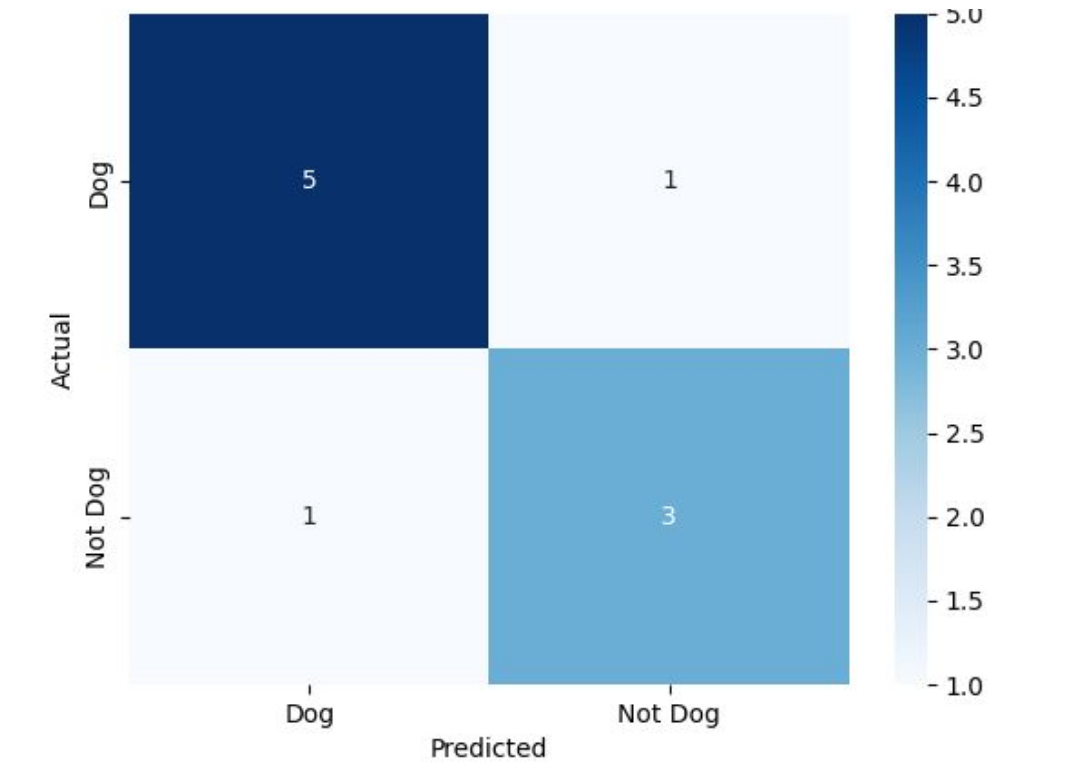
\includegraphics[width=\linewidth]{Pictures/multiclass_2.png}
    \end{subfigure}
\end{figure}
$$
\text{precision}=\frac{\text{TP}}{\text{TP}+\text{FP}}=\frac{\text{\# True positives}}{\text{\# Predicted positives}}
$$
The precision measures: of all items predicted as positive ($\hat{y}=1$), what fraction is actually positive ($y=1$)?
It quantifies how "precise" your classifier is in identifying positives. For example, of all emails flagged as spam, how many actually are?
\textbf{Maximizing precision = minimizing false positives.}
$$
\text{recall}=\frac{\text{TP}}{\text{TP}+\text{FN}}
$$
The recall measures: of all actual positives ($y=1$), what fraction is predicted as positive ($\hat{y}=1$)?
It quantifies how good your classification is covering all positive cases. For example, of all actual COVID-19 cases, how many are diagnosed by a specific test?
\textbf{Maximizing recall = minimizing false negatives.} 
$$
\text{F1 score}=2\times\frac{\text{precision}\times\text{recall}}{\text{precision}+\text{recall}}
$$
The F1 score is the harmonic mean of precision and recall. It balances the importance of precision and recall, and is preferable to accuracy for class-imbalanced datasets.
\begin{itemize}
    \item When the precision and recall are both 1 $\Rightarrow$ F1 = 1.
    \item When the precision and recall are similar, F1 will be close to both.
    \item When the precision and recal are far apart, F1 will be closer to whichever is worse.  
\end{itemize}
\begin{figure}[H]
    \centering
    \begin{subfigure}{0.7\textwidth}
        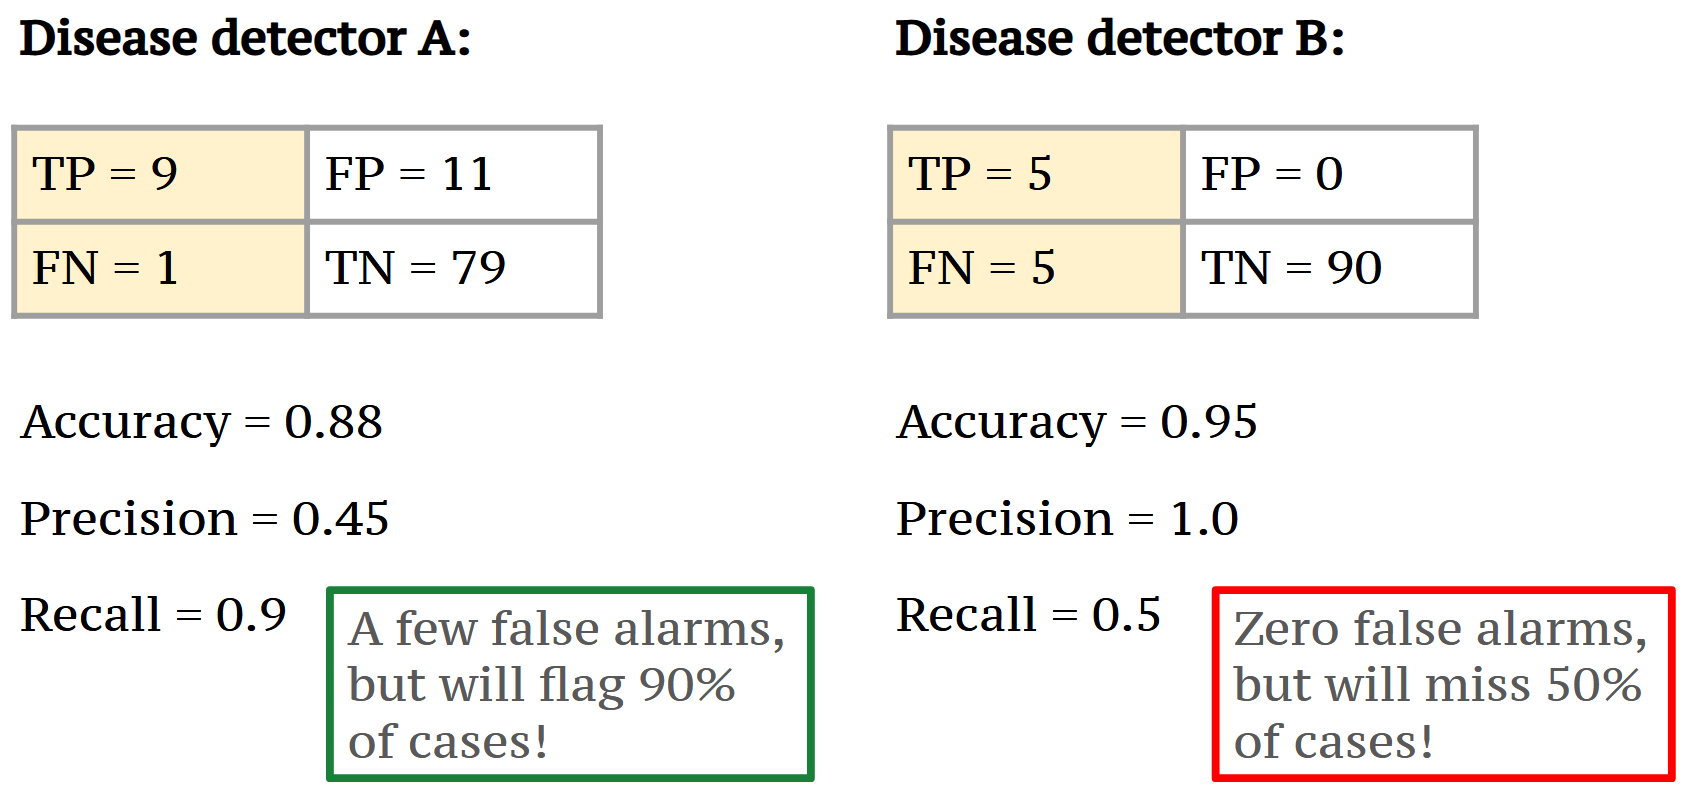
\includegraphics[width=\linewidth]{Pictures/multiclass_3.png}
    \end{subfigure}
\end{figure}
$\quad$\\[-1em]
Confusion matrices can also be generalized to multi-class classification.
Calculate the precision, recall, F1 for class $c\in\{1,\dots,K\}$ by treating each class in turn as the positive class and the rest as negative.
\begin{figure}[H]
    \centering
    \begin{subfigure}{0.4\textwidth}
        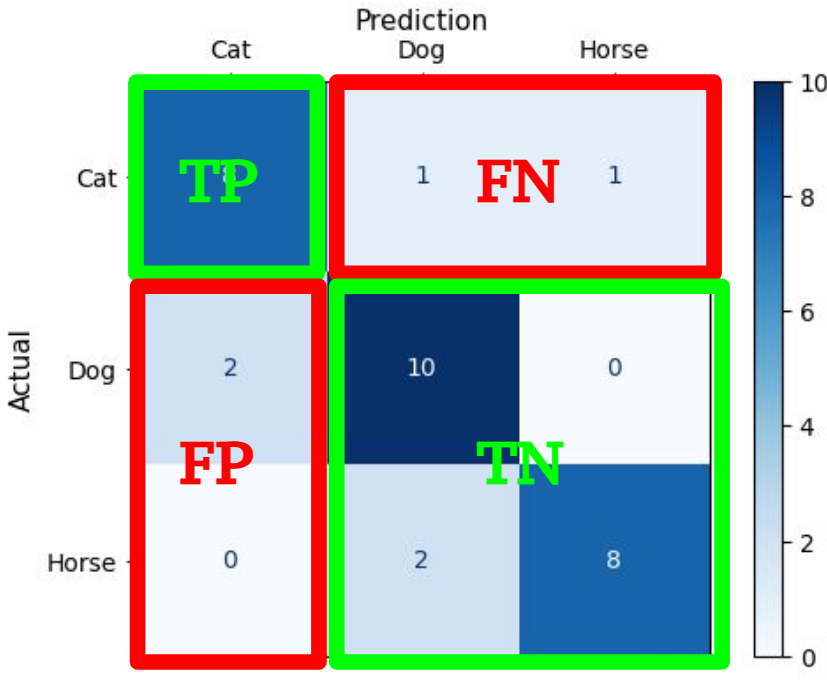
\includegraphics[width=\linewidth]{Pictures/multiclass_4.png}
    \end{subfigure}
\end{figure}

\subsection{Perceptron modelling decison}
\subsubsection{Parameter initialization}
Parameters are learned throughthe perceptron learning rule, but what are their initial values? In machine learning, parameters are randomly initialized.
Initialization is only the starting point. Parameters are adjusted during training anyway to improve performance.
How you initialize parameters affects convergence speed and the path the perceptron takes during training.
While the perceptron will eventually converge (if linearly separable), good initialization can make convergence faster and smoother.
\begin{figure}[H]
    \centering
    \begin{subfigure}{\textwidth}
        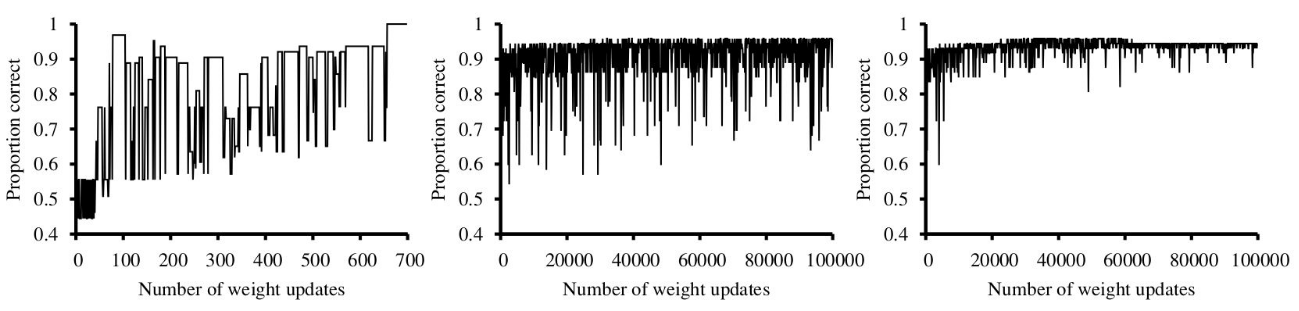
\includegraphics[width=\linewidth]{Pictures/PMD_1.png}
    \end{subfigure}
\end{figure}
$\quad$\\[-1em]
There are options for initializing perceptron weights (and bias):
\begin{itemize}
    \item \textbf{Zero initialization:}
    \begin{itemize}
        \item All parameters start at 0.
        \item Works for binary perceptron, but not always for multi-class perceptrons.
        \item \begin{lstlisting} 
np.zeros(n_inputs)
\end{lstlisting}
    \end{itemize}
    \item \textbf{Small constant initialization:}
    \begin{itemize}
        \item All parameters start at a small constant value, e.g. 0.01
        \item \begin{lstlisting}
np.full(n_inputs, 0.01)
\end{lstlisting}
    \end{itemize}
    \item \textbf{Uniform random initialization:}
    \begin{itemize}
        \item Parameters are random values drawn from a uniform distribution.
        \item \begin{lstlisting}
np.random.uniform(-0.01, 0.01, n_inputs)            
\end{lstlisting}
    \end{itemize}
    \item \textbf{Gaussian initialization:}
    \begin{itemize}
        \item Parameters are random values drawn from a normal distribution.
        \item \begin{lstlisting}
np.random.normal(0.0, 0.01, n_inputs)            
\end{lstlisting}
    \end{itemize}
\end{itemize}
\subsubsection{Feature representation}
The big question is: how do you represent data points? For this, we use multi-dimensional vectors. Each inputs in the dataset $\{(x_1,y_1),(x_2,y_2),\dots,(x_n,y_n)\}$ is represented as an $n$-dimensional vector. The choice of features $x_{i1},x_{i2},\dots,x_{in}$ will be different for different tasks/domains.
For image processing tasks (e.g. MNIST classification) you can flatten the pixel matrix into a vector. A $28\times 28$ image is a 784-dimensional vector.
\begin{figure}[H]
    \centering
    \begin{subfigure}{0.8\textwidth}
        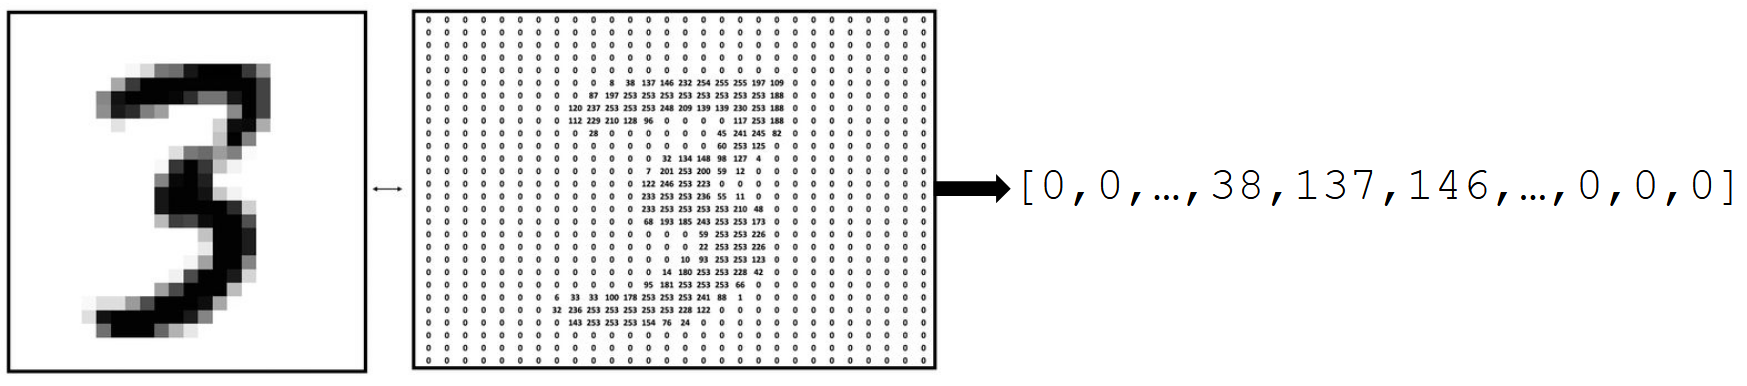
\includegraphics[width=\linewidth]{Pictures/PMD_2.png}
    \end{subfigure}
\end{figure}
$\quad$\\[-1em]
For some taks, color information could be worth including. Color images store RGB (red-green-blue) values. The earliest way to represent the image as a vector is to flatten the RGB values.
\begin{figure}[H]
    \centering
    \begin{subfigure}{0.7\textwidth}
        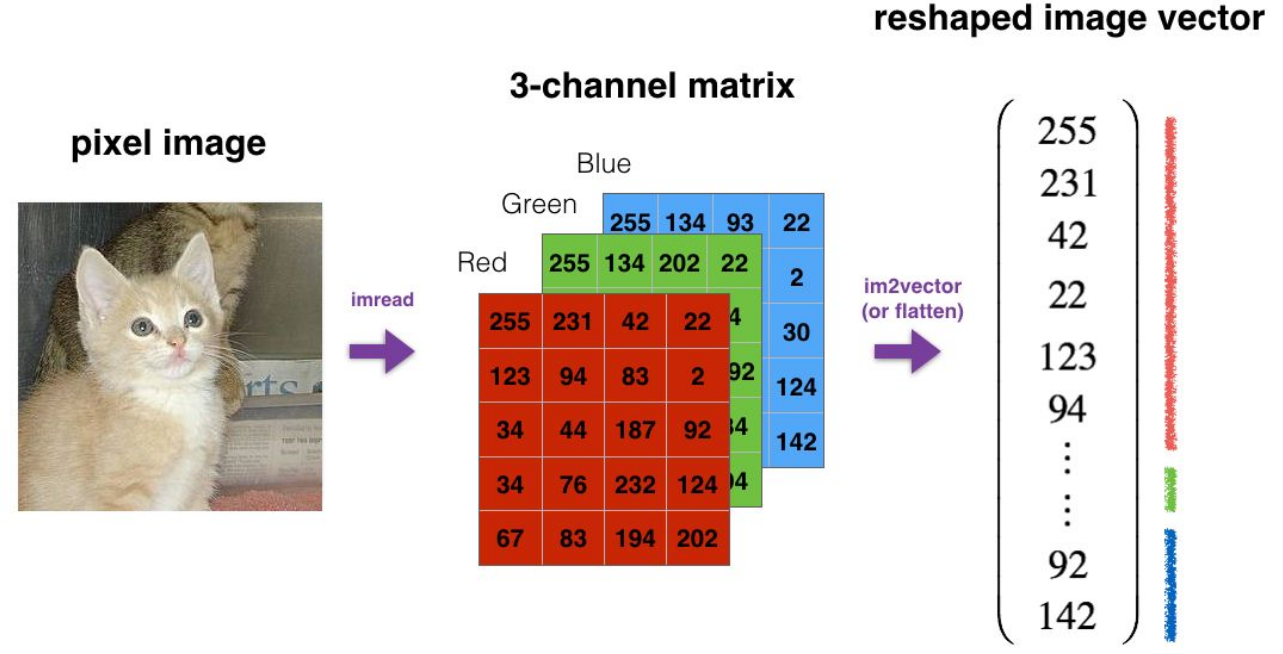
\includegraphics[width=\linewidth]{Pictures/PMD_3.png}
    \end{subfigure}
\end{figure}
$\quad$\\[-1em]
Features can have very different scales, e.g. $x_1\in[0,1]$ or $x_2\in[0,1000]$.
\begin{itemize}
    \item Distances and dot products are dominated by large-scale features.
    \item For classifiers based on Euclidean distance (e.g. k-nearest neighbor), decisions can mostly eflect large features, ignoring the smaller one.
    \item For perceptrons, the weight updates can be skewed towards large-magnitude features.
    \item As a consequence, it results in slow/unstable convergence and poor decision boundaries.
\end{itemize}
\subsubsection{Normalization (min-max)}
With min-max scaling, we rescale each feature individually to a fixed range, typically $[0,1]$.
$$
x_{ij}^{\text{max}}=\frac{x_{ij}-\text{min}_l(x_{lj})}{\text{max}_l(x_{lj})-\text{min}_l(x_{lj})}
$$
where:
\begin{itemize}
    \item $x_{ij}$ is the value of feature $j$ for data point $i$.
    \item $\text{max}_l(x_{lj})$ is the maximum value of feature $j$ across all data points.
    \item $\text{min}_l(x_{lj})$ is the minimum value of feature $j$ across all data points.
\end{itemize}
This keeps all inputs in the same range. Rather intuitive for image pixels (0-255 is mapped to 0-1).
\begin{figure}[H]
    \centering
    \begin{subfigure}{0.8\textwidth}
        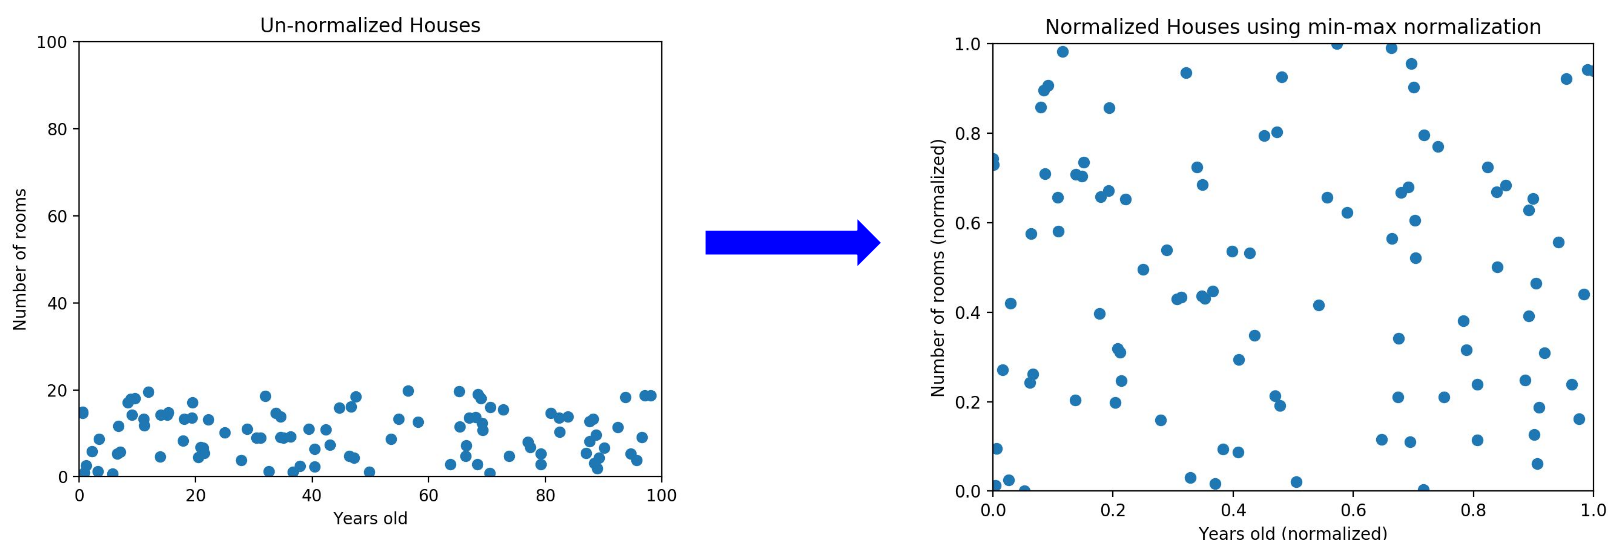
\includegraphics[width=\linewidth]{Pictures/PMD_4.png}
    \end{subfigure}
\end{figure}
\begin{warning}[Important]
Compute $\text{min}_l(x_{lj})$ and $\text{max}_l(x_{lj})$ from the \textbf{training set only.} Apply to the training, validation and test sets.
\end{warning}
\subsubsection{Normalization (Z-score)}
With Z-score normalization, we center and scale features to habe a mean of 0 and variance of 1.
$$
x_{ij}^{\text{new}}=\frac{x_{ij}-\bar{x}_j}{\sigma_j}
$$
where:
\begin{itemize}
    \item $x_{ij}$ is the value of feature $j$ for a data point $i$.
    \item $\bar{x}_j$ is the mean value of feature $j$ in the training data.
    \item $\sigma_j$ is the standard deviation of feature $j$ in the training data.
\end{itemize}
It is robust when featues have different units, with measurements producing varying feature distributions e.g. age vs height. Also robust when outliers are present.
\begin{figure}[H]
    \centering
    \begin{subfigure}{0.8\textwidth}
        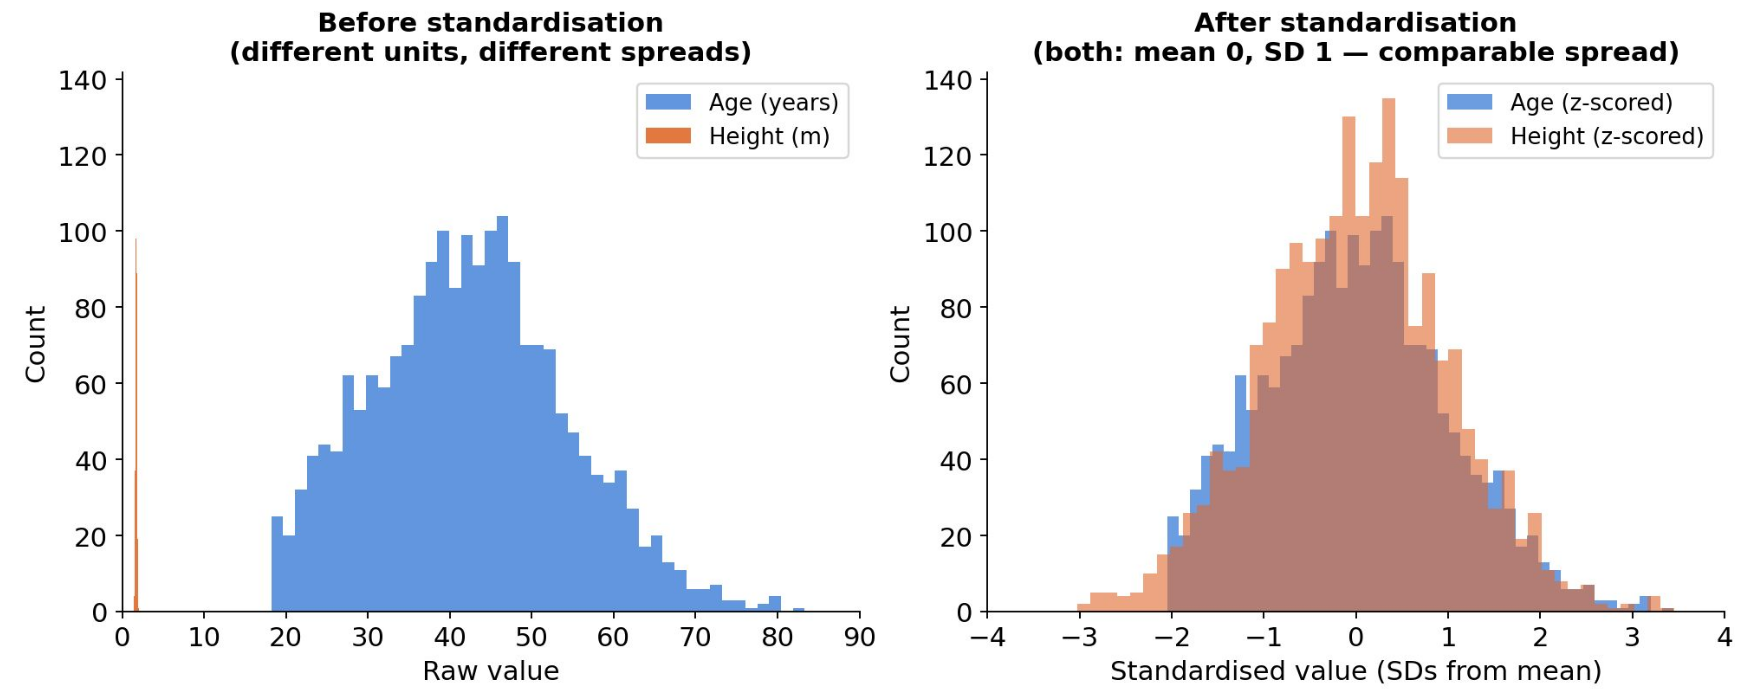
\includegraphics[width=\linewidth]{Pictures/PMD_5.png}
    \end{subfigure}
\end{figure}
\subsubsection{Overfitting}
Overfitting is when your model is fitting the details of the training data so closely that the model doesn't generalize well to the test set. This happens when the model is over-parameterized. It has more parameters that required to model the data.
\begin{figure}[H]
    \centering
    \begin{subfigure}{0.8\textwidth}
        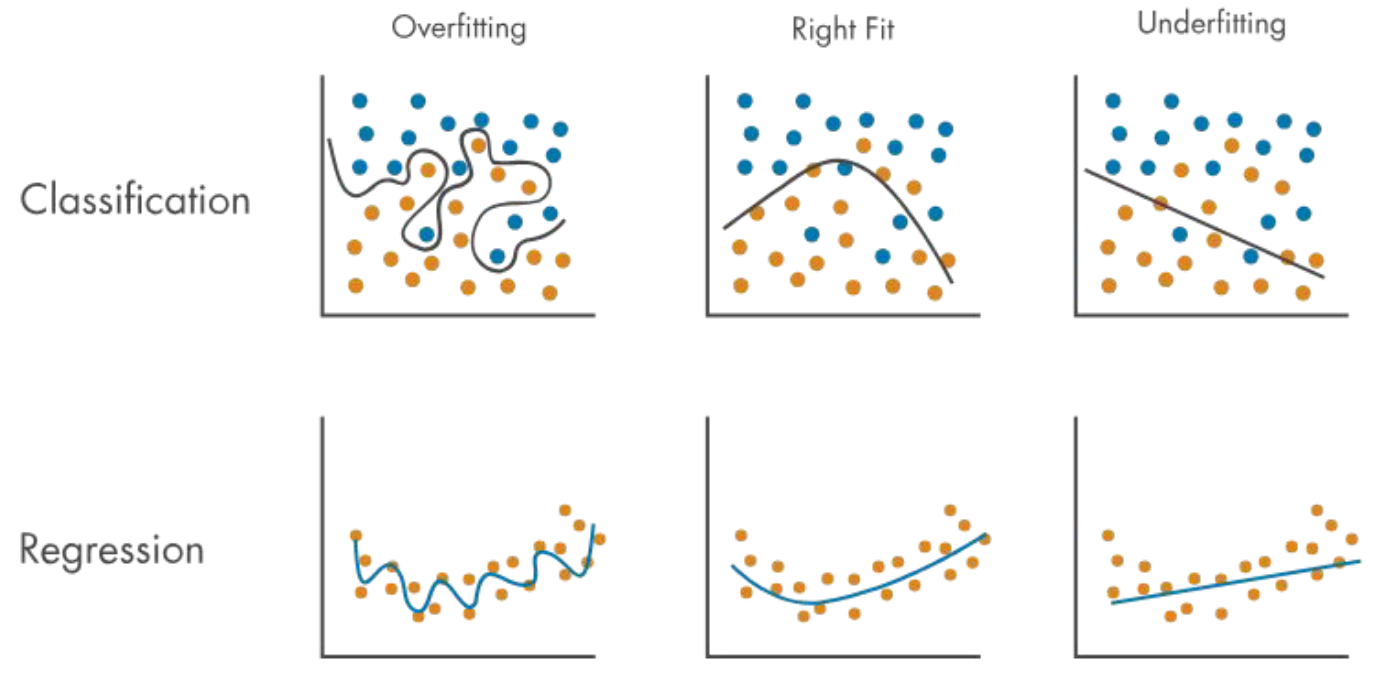
\includegraphics[width=\linewidth]{Pictures/PMD_6.png}
    \end{subfigure}
\end{figure}
How can overfitting happen for a perceptron?
\begin{itemize}
    \item Each weight $w_i$ corresponding to and input feature $x_i$.
    \item During training, the value $w_i$ is learned such that $w_ix_i$ will contribute to improving the accuracy for examples in the training set.
    \item If a feature $x_i$ happens to only occur in one class in the training data, the model could learn a very high weight $w_i$ and perfectly predict $y$.
    \item In this case, the model will fail to generalize to the test set without this feature.
\end{itemize}
Overfitting will result in a high (even perfect) accuracy on training data, bu a low accuracy on validation and test data. That's why it's important to track validation performance during training.
\subsubsection{Early stopping}
Validation performance typically improves first, then (sometimes) degrades as overfitting sets in. After this, improving the model's fit to the training data comes at the expense of generalization.
Early stopping is when we stop training when the performance on a held-out validation dataset stops improving, to avoid overfitting. It is commonly used in machine learning to prevent overfitting.
\begin{figure}[H]
    \centering
    \begin{subfigure}{0.6\textwidth}
        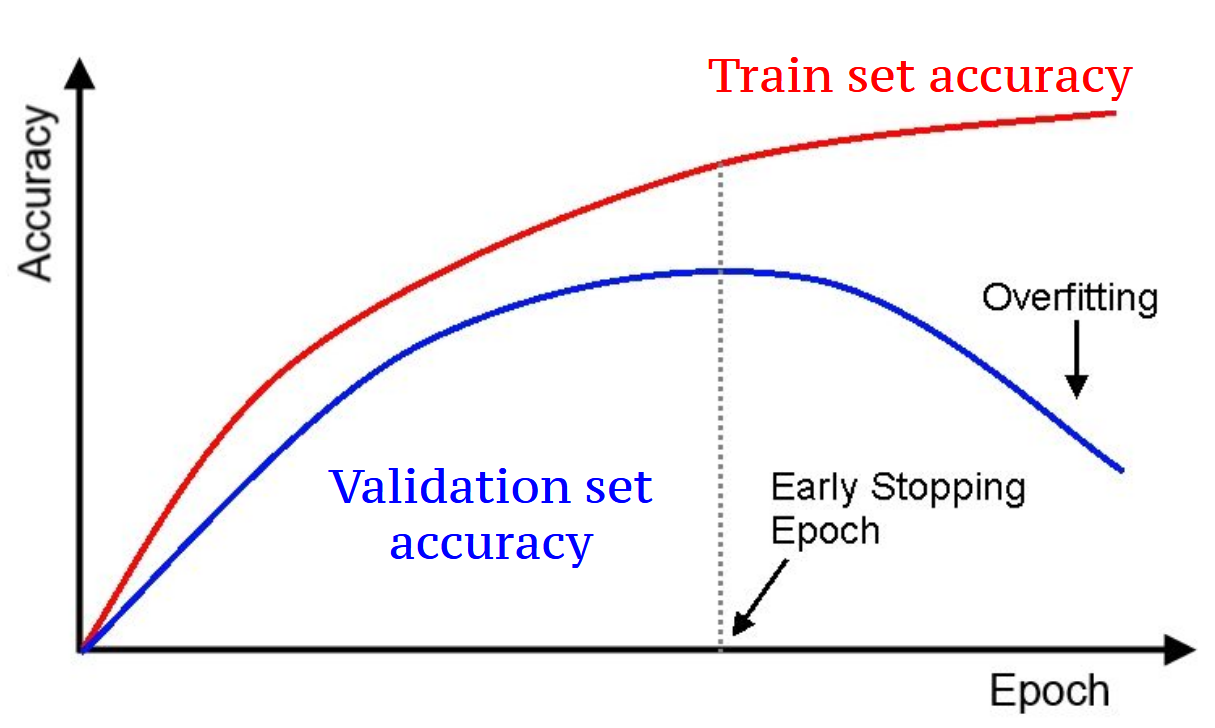
\includegraphics[width=\linewidth]{Pictures/PMD_7.png}
    \end{subfigure}
\end{figure}
\subsubsection{Validation set}
\begin{definition}[Validation set]
A \textbf{validation set} is a held-out set not used for training the model. It's purpose is to estimate how the model will generalize. It is used during and after training.
\end{definition}
$\quad$\\[-1em]
\textbf{Use 1: During training} \\
It is used to track performance on unseen data while training. It helps to detect overfitting and enables early stopping. The validation curves is the "progress report."
\\\\
\textbf{Use 2: After training (hyperparameter tuning)} \\
For each hyperparameter setting, we train the model until completion, and then record the final/best accuracy achieved. Each hyperparameter setting has one final validation score. 
Compare this across different settings to choose the best hyperparameters.
\begin{enumerate}
    \item Choose your stopping criteria.
    \item Choose the range of your hyperparameter search.
    \begin{itemize}
        \item learning rate e.g. $\{0.01, 0.05, 0.1, 0.5\}$.
        \item initialization e.g. $\{\text{zeros, uniform, gaussian}\}$.
        \item feature normalization e.g. $\{\text{none, normalization, standardization}\}$.
    \end{itemize}
    \item Train the model for each possible combination of hyperparameters, saving the final/best validation accuracy. This is typically called grid search.
\end{enumerate}
\begin{figure}[H]
    \centering
    \begin{subfigure}{0.6\textwidth}
        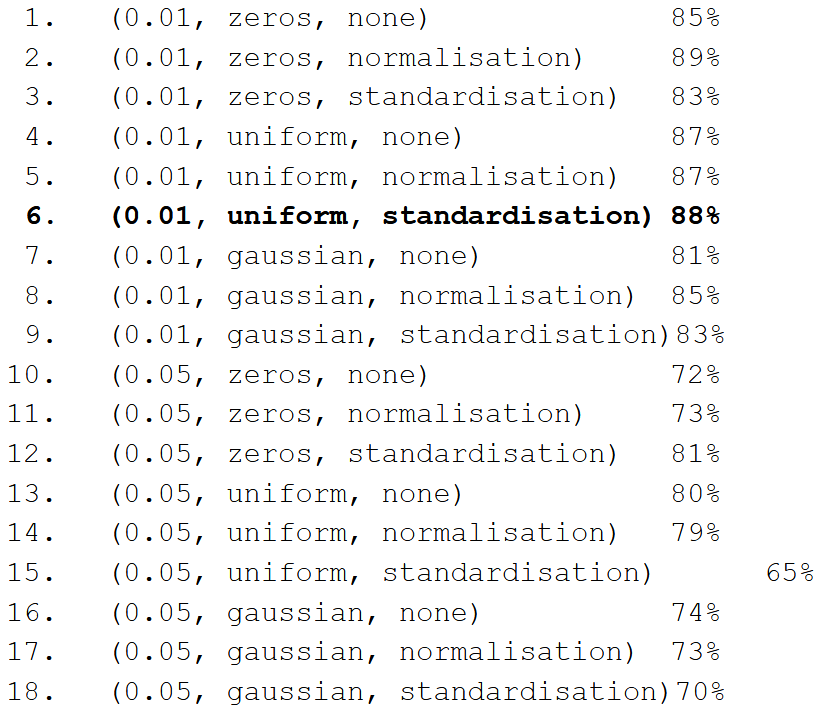
\includegraphics[width=\linewidth]{Pictures/PMD_8.png}
    \end{subfigure}
\end{figure}

\subsection{Simple linear regression}
A simple linear regression model predicts the output as a linear function of one input feature $x$: $y=wx+b$, otherwise known as a straight line function. Changes in $x$ imply a proportional change in $y$. Even if the relationship is not perfectly linear, linear regression can still be effective as an approximation or baseline model.
\begin{figure}[H]
    \centering
    \begin{subfigure}{0.8\textwidth}
        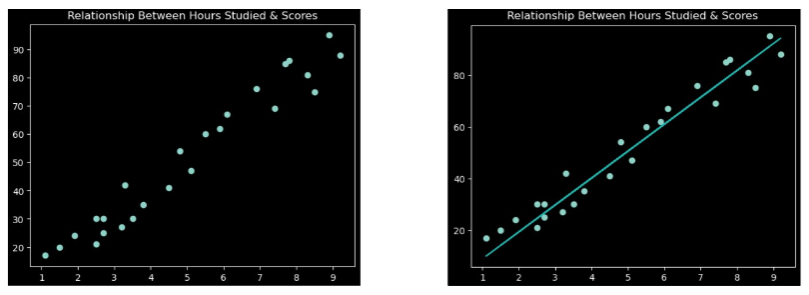
\includegraphics[width=\linewidth]{Pictures/SLR_1.png}
    \end{subfigure}
\end{figure}

\subsubsection{Loss function}
For each input, linear regression produces an estimate $\hat{y}_i=w\cdot x_i+b$. We want to set $w$ and $b$ to minimize the distance between our estimate $\hat{y}_i$ (prediction) and the true $y_i$. We want to minimize this distance/error across our entire training set $\{(x_1,y_1),(x_2,y_2),\dots,(x_N,y_N)\}$.
\\[1em]
A principled way to define the learning problem is with a loss function (also known as a cost function): $L(\hat{y}_i,y_i)$ measuring how close the model prediction $\hat{y}_i$ is to the observed data $y_i$. If the model fits the data well, so that $y_i\approx \hat{y}_i$, then the loss function should take a small value, and vice versa. For this, we can use the squared error loss.
\begin{figure}[H]
    \centering
    \begin{subfigure}{0.5\textwidth}
        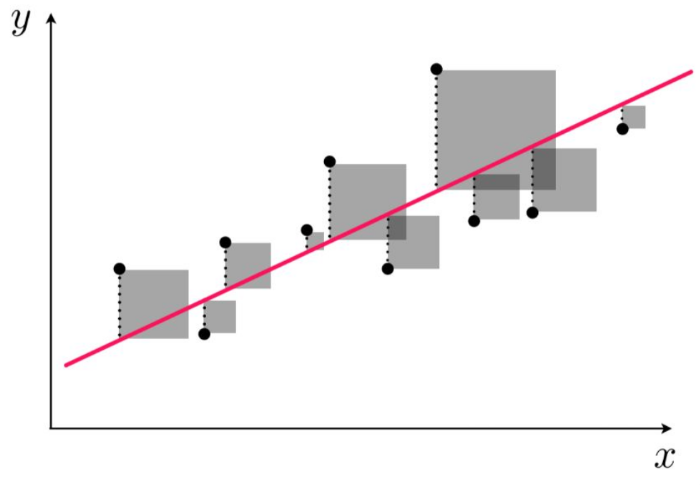
\includegraphics[width=\linewidth]{Pictures/SLR_2.png}
    \end{subfigure}
\end{figure}
$\quad$\\[-1em]
The squared error loss measures how good your linear regression model with parameters $w,b$ fits the data. For a single data point $(x_i,y_i)$:
\begin{align*}
    L(\hat{y}_i,y_i)&=(y_i-\hat{y}_i)^2 \\
    &=(y_i-f(x_i;w,b))^2 \\
    &=(y_i-(w\cdot x+b))^2 \\
    &=(y_i-w\cdot x-b)^2
\end{align*}
We want to find the weight that minimizes the loss, averaged over all examples in our training set.
$$
\boxed{J(w,b)=\frac{1}{N}\sum_{i=1}^{N}L(\hat{y}_i,y_i)}
$$
\begin{note}[Note: Why as a function of $w$ and $b$?]
These are the variables we want to learn!
\end{note}
$\quad$\\[-1em]
All examples $(x_i,y_i)$ in the function are determined by whatever is in the training set. This is out of our control. Now, we want to find:
$$
\hat{w},\hat{b}=\underset{w,b}{\text{argmin}}J(w,b)
$$
For linear regression, the loss function (mean squared error) is convex. This means it has a single global minimum and no local minima. Linear regression has a closed form solution. The question is, how do we find $\hat{w},\hat{b}=\underset{w,b}{\text{argmin}}J(w,b)$?
\begin{enumerate}
    \item Take the partial derivative of $J$ with respect to $w$ and $b$.
    \item Set the partial derivative equal to 0.
    \item Solve for $w$ and $b$.
\end{enumerate}
\begin{note_special}[Derivation]
\textbf{Derivation w.r.t $b$:}
\begin{align*}
    \frac{\partial}{\partial b}J(w,b)&=\frac{\partial}{\partial b}\frac{1}{N}\sum_{i=1}^{N}(y_i-wx_i-b)^2 \\
    &=\frac{-2}{N}\sum_{i=1}^{N}(y_i-wx_i-b) \\
    0&=\sum_{i=1}^N(y_i-wx_i-b) \quad\text{(Setting equal to 0)} \\
    0&=\sum_{i=1}^{N}y_i -w\sum_{i=1}^{N}x_i-Nb \\
    \hat{b}&=\bar{y}-\hat{w}\bar{x}
\end{align*}
\textbf{Derivation w.r.t $w$:}\\
Before differentiating w.r.t $w$, substitute this expression for $b$ back into the cost so that $J$ becomes a function of $w$ only:
$$
J(w)=\frac{1}{N}\sum_{i=1}^{N}\Big[y_i-wx_i-(\bar{y}-w\bar{x})\Big]^2=\frac{1}{N}\sum_{i=1}^{N}\Big[(y_i-\bar{y})-w(x_i-\bar{x})\Big]^2
$$
Now differentiate w.r.t $w$:
$$
\frac{d}{dw}J(w)=\frac{-2}{N}\sum_{i=1}^{N}\big[(y_i-\bar{y})-w(x_i-\bar{x})\big]\big[(x_i-\bar{x})\big]
$$
Set the derivative to 0 and simplify:
\begin{align*}
    0&=\frac{-2}{N}\Big[\sum_{i=1}^{N}(y_i-\bar{y})(x_i-\bar{x})-w\sum_{i=1}^{N}(x_i-\bar{x})^2\Big] \\
    w\sum_{i=1}^{N}(x_i-\bar{x})^2&=\sum_{i=1}^{N}(y_i-\bar{y})(x_i-\bar{x}) \\
    \hat{w}&=\frac{\sum_{i=1}^{N}(y_i-\bar{y})(x_i-\bar{x})}{\sum_{i=1}^{N}(x_i-\bar{x})^2}
\end{align*}
\end{note_special}

\subsection{Logistic regression}
\subsubsection{Probability basics}
\begin{itemize}
    \item $P(A)$: probability of event $A$.
    \item $P(A^c)$: probability of event $A$ not happening.
    \item $P(A|B)$: probability of $A$ given $B$ (conditional probability).
    \item For any event $A$, $0\leq P(A)\leq 1$.
    \item Let $S$ be the sample space of all possible events, then $P(S)=1$.
    \item For any event $A$, $P(A^c)=1-P(A)\iff P(A)=1-P(A^c)$.
\end{itemize}

\subsubsection{Discriminative classifier}
Discriminative models learn boundaries between classes. For example, suppose we are classifying cat vs. dog images. The input $x$ is the image (matrix of pixel values). The output $y$ is the class (either cat or dog).
The goal of classification is to find the correct class $y$ given input $x$. To classify, we compute: $y=\underset{y\in C}{\text{argmax}}P(y|x)$.

\subsubsection{Logistic regression}
We introduce the sigmoid function:
$$
\sigma(z)=\frac{1}{1+e^{-z}}
$$
\begin{figure}[H]
    \centering
    \begin{subfigure}{0.5\textwidth}
        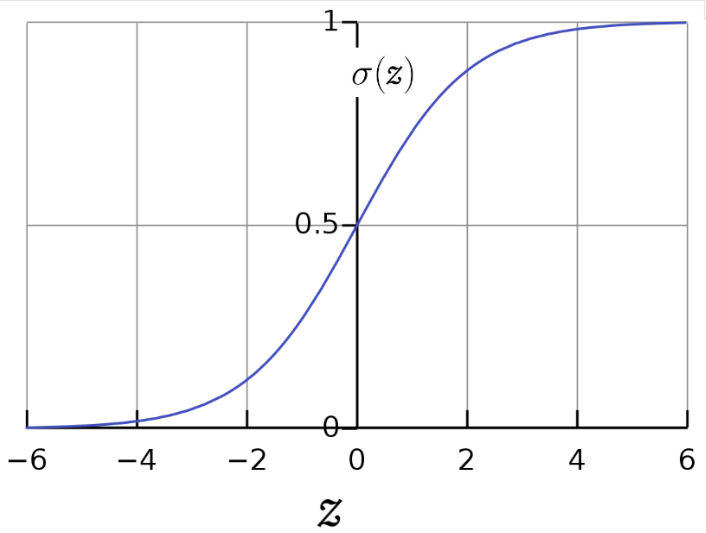
\includegraphics[width=\linewidth]{Pictures/LR_1.png}
    \end{subfigure}
\end{figure}
$\quad$\\[-1em]
The sigmoid function is called a logistic function. It squeezes any input value between 0 and 1. To classify the input $\mathbf{x}$:
\begin{itemize}
    \item Compute the weighted sum, $z=\sum w_ix_i+b=\mathbf{w}\cdot\mathbf{x}+b$.
    \item Pass $z$ through the sigmoid function, $\sigma(\mathbf{w}\cdot\mathbf{x}+b)$.
    \item Treat the result as a probability. $$ P(y=1|\mathbf{x})=\sigma(\mathbf{w}\cdot\mathbf{x}+b)=\frac{1}{1+\text{exp}(-\mathbf{w}\cdot\mathbf{x}-b)} $$
\end{itemize}
A key property of the sigmoid function: $1-\sigma(z)=\sigma(-z)$.
\begin{note_special}[Derivation]
\begin{align*}
    P(y=0|\mathbf{x})&=1-\sigma(\mathbf{w}\cdot\mathbf{x}+b) \\
    &=1-\frac{1}{1+\text{exp}(-\mathbf{w}\cdot\mathbf{x}-b)} \\
    &=\frac{\text{exp}(-\mathbf{w}\cdot\mathbf{x}-b)}{1+\text{exp}(-\mathbf{w}\cdot\mathbf{x}-b)}\times\frac{\text{exp}(\mathbf{w}\cdot\mathbf{x}+b)}{\text{exp}(\mathbf{w}\cdot\mathbf{x}+b)} \\
    &=\frac{1}{1+\text{exp}(\mathbf{w}\cdot\mathbf{x}+b)} \\
    &=\sigma(-\mathbf{w}\cdot\mathbf{x}-b)
\end{align*}
\end{note_special}
$\quad$\\[-1em]
Now, we have a way to compute both $P(y=1|\mathbf{x})$ and $P(y=0|\mathbf{x})$. We can now make decisions:
$$
\text{decision}(\mathbf{x})=\begin{cases}
    1 & \text{if }P(y=1|\mathbf{x})>0.5 \\
    0 & \text{otherwise}
\end{cases}
$$
The decision boundary of $P(y|x)=0.5$ is defined where $\mathbf{w}\cdot\mathbf{x}+b=0$. This is the default decision boundary in logistic regression. However, you can specify a different decision boundary to suit your task.
\begin{itemize}
    \item Choose a higher value, like $P(y=1|\mathbf{x})>0.9$, if you want the model to be confident before flagging an instance of a positive class.
    \item Choose a lower value, like $P(y=1|\mathbf{x})>0.2$, if you don't want to risk missing instances of the positive cass (e.g. medical diagnosis).
\end{itemize}

\subsubsection{Example}
Predict if a fire weather warning should be announced.
\begin{itemize}
    \item $x_1$: temperature in $C^\circ$.
    \item $x_2$: wind speed in km/h.
    \item $y=0$: no warning needed.
    \item $y=1$: warning needed.
\end{itemize}
Suppose the weights are $\mathbf{w}=[0.1,0.05]$ and the bias term is $b=-5$. For an input vector $\mathbf{x}=[25,60]$,
\begin{align*}
    P(y=1|\mathbf{x})&=\sigma(\mathbf{w}\cdot\mathbf{x}+b)=\sigma((0.1)(25)+(0.05)(60)-5)=\sigma(0.5)=0.622 \\
    P(y=0|\mathbf{x})&=1-P(y=1|\mathbf{x})=1-0.622=0.378
\end{align*}
Since $P(y=1|\mathbf{x})=0.622>0.5$, a warning should be given.

\subsection{Cross-entropy loss}
\subsubsection{Log probabilities}
\begin{definition}[Log probability]
    A log probability is a logarithm of a probability value, $\log P(X)$. This represents probabilities on a logarithmic scale $(-\infty,0]$ instead of the usual $[0,1]$ probability interval.
\end{definition}
$\quad$\\[-1em]
A useful property of log properties:
$$
\log P(ABC)=\log(P(A)\times P(B)\times P(C))=\log P(A)+\log P(B)+\log P(C)
$$

\subsubsection{Loss function}
We use conditional \textbf{maximum likelihood estimation}:
\begin{itemize}
    \item Find parameters that \textbf{maximize the probability of the true labels} in the training data given the observations.
    \item For binary classification, since there are 2 discrete outcomes, we can express the classifier's probability of the true label $y$ as:
$$
P(y|\mathbf{x})=\hat{y}^y(1-\hat{y})^{1-y}
$$
    \item If $y=1$, this simplifies to $\hat{y}$ which is $P(y=1|\mathbf{x})$.
    \item If $y=0$, this simplifies to $1-\hat{y}$ which is $P(y=0|\mathbf{x})$.
\end{itemize}
$\quad$\\[-1em]
We can rewrite this in terms of log probabilities:
\begin{align*}
    \log P(y|\mathbf{x})&=\log\big[\hat{y}^y(1-\hat{y}^{1-y})\big] \\
    &=y\log\hat{y}+(1-y)\log(1-\hat{y})
\end{align*}
We can then turn this into a loss function to be minimized by using the negative log likelihood. This is called the \textbf{cross-entropy loss} between the prediction and the true class.
\begin{align*}
    L_{\text{CE}}(\hat{y},y)&=-\log P(y|\mathbf{x}) \\
    &=-\big[y\log\hat{y}+(1-y)\log(1-\hat{y})\big] \\
    &=-\big[y\log[\sigma(\mathbf{w}\cdot\mathbf{x}+b)]+(1-y)\log[\sigma(-\mathbf{w}\cdot\mathbf{x}-b)]\big]
\end{align*}
By minimizing this loss, we maximize the probabilities assigned to the true labels by the logistic regression model.

\subsubsection{Example}
Predict if a fire weather warning should be announced.
\begin{itemize}
    \item $x_1$: temperature in $C^\circ$.
    \item $x_2$: wind speed in km/h.
    \item $y=0$: no warning needed.
    \item $y=1$: warning needed.
\end{itemize}
Suppose the weights are $\mathbf{w}=[0.1,0.05]$ and the bias term is $b=-5$. \\\\ 
For an input vector $\mathbf{x}=[25,60]$ and true label $y=1$:
\begin{flalign*}
    P(y=1|\mathbf{x})&=\sigma(\mathbf{w}\cdot\mathbf{x}+b)=0.622 &\\
    L_{\text{CE}}(\hat{y},{y})&=-\log P(y=1|\mathbf{x})=-\log 0.622 = 0.206 &
\end{flalign*}
For an input vector $\mathbf{x}=[25,60]$ and true label $y=0$:
\begin{flalign*}
    P(y=0|\mathbf{x})&=1-\sigma(\mathbf{w}\cdot\mathbf{x}+b)=0.378 &\\
    L_{\text{CE}}(\hat{y},y)&=-\log P(y=0|\mathbf{x})=-\log 0.378=0.423 &
\end{flalign*}
Since the loss of true label $y=1$ is lower, we should give a warning.
\begin{note}[Note]
The loss is higher if the model is wrong. Lower probabilities assigned to the true class implies a higher loss.
\end{note}

\subsubsection{Objective function}
Given the cross-entropy loss, we want to minimize this loss on average across our training set:
$$
\boxed{\frac{1}{N}\sum_{i=1}^{N}L_{\text{CE}}(\hat{y}_i,y_i)}
$$
If we can adjust parameters $\mathbf{w}$ and $b$ to lower the loss over all instances in the training set, we will have a good classifier. This is the essence of modern machine learning and deep learning.

\subsubsection{Optimization}
Let the loss function be parameterized by parameters $\theta=(\mathbf{w},b)$. We represent $\hat{y}$ as $f(\mathbf{x};\theta)$. We want to find parameters that minimize the loss averaged over all examples in our training set.
$$
\hat{\theta}=\underset{\theta}{\text{argmin}}\hspace{2pt}\frac{1}{N}\sum_{i=1}^{N}L_{\text{CE}}(f(\mathbf{x};\theta),y_i)
$$ 
There is \textbf{no closed form solution} for finding minimizing weights for logistic regression. Instead, we will use an iterative method called gradient descent.

\subsection{Gradient descent}
\begin{definition}[Gradient descent]
Gradient descent is an optimization algorithm that iteratively updates parameters by moving in the opposite direction of the gradient of the loss function, in order to minimize the loss.
\end{definition}
\subsubsection{Loss function}
We want parameters $\mathbf{w},b$ that minimize loss averaged over $m$ examples in our training set. We denote the average loss as $J(\mathbf{w},b)$ with $\hat{y}_i=f(\mathbf{x}_i;\mathbf{w},b)$ written as a function of inputs and parameters.
$$
J(\mathbf{w},b)=\frac{1}{m}\sum_{i=1}^{m}\big[y_i\log\sigma(\mathbf{w}\cdot\mathbf{x}_i+b)+(1-y_i)\log[1-\sigma(\mathbf{w}\cdot\mathbf{x}_i+b)]\big]
$$
Now, we want to find:
$$
\hat{\mathbf{w}},\hat{b}=\underset{\mathbf{w},b}{\text{argmin}}\hspace{2pt}J(\mathbf{w},b)
$$

\subsubsection{Optimization}
For logistic regression, the loss function is convex. Gradient descent from any point is guarenteed to find the minimum. Here is a visualization for a single scalar $w$: Given the current $w$, move in the reverse direction from the function slope.
\begin{figure}[H]
    \centering
    \begin{subfigure}{\textwidth}
        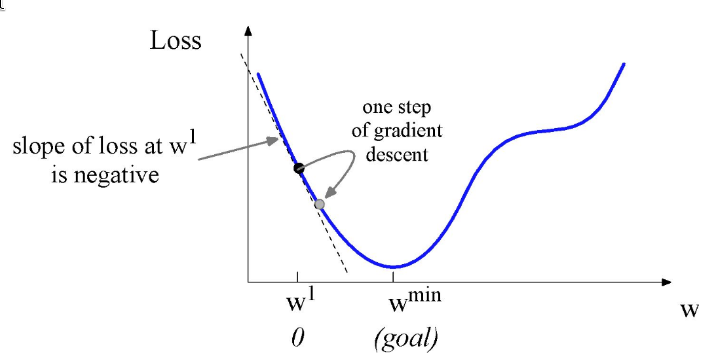
\includegraphics[width=\linewidth]{Pictures/GD_1.png}
    \end{subfigure}
\end{figure}
$\quad$\\[-1em]
The loss is a function of multiple parameters $w_1,\dots,w_n,b$:
$$
L_{\text{CE}}=-\big[y\log\sigma(\mathbf{w}\cdot\mathbf{x}+b)+(1-y)\log[1-\sigma(\mathbf{w}\cdot\mathbf{x}+b)]\big]
$$
The gradient of this loss with respect to the parameters $\theta$ will be a vector of partial derivatives.
$$
\nabla_{\theta}L=\frac{\partial L}{\partial \theta}=\begin{bmatrix}
    \frac{\partial L}{\partial w_1} \\
    \frac{\partial L}{\partial w_2} \\
    \vdots \\
    \frac{\partial L}{\partial w_n} \\
    \frac{\partial L}{\partial b}
\end{bmatrix}
$$
For models with $n$-dimensional weight vectors:
\begin{itemize}
    \item For each dimension $w_i$, the gradient component $i$ tells us the slope w.r.t that parameter.
    \item We express the slope as the partial derivative of $L$ w.r.t $w_i$.
    \item The gradient is defined as the vector of these partial derivatives.
\end{itemize}

\subsubsection{Learning rate}
$$
\mathbf{w}^{t+1}=\mathbf{w}^t-\eta\frac{d}{dw}L(f(\mathbf{x};\mathbf{w}),y)
$$
The gradient tells us:
\begin{itemize}
    \item \textbf{Sign:} which way to move (left, right, up, down).
    \item \textbf{Magnitude:} how steep/big the update is.
\end{itemize}
To control the step size, the value of the gradient is weighted by a learning rate $\eta$. A higher value of $\eta$ means $\mathbf{w}$ changes faster. This is considered a hyperparameter.
\begin{itemize}
    \item If the learning rate is too high, it will take big steps and overshoot.
    \item If the learning rate is too low, it will take too long to converge.
\end{itemize}

\subsubsection{Optimization (continued)}
How do we find $\hat{\theta}=\underset{\theta}{\text{argmin}}\hspace{2pt}\frac{1}{m}\sum_{i=1}^{m}L_{\text{CE}}(f(\mathbf{x};\theta), y_i)$? We do the following iteratively:
\begin{itemize}
    \item Compute the derivative of the loss function with respect to the parameters.
    \item Update the parameters to move in the opposite direction of the gradient.
\end{itemize}
The partial derivatives for logistic regression:
$$
\boxed{\frac{\partial L}{\partial w_i}=[\sigma(\mathbf{w}\cdot\mathbf{x}+b)-y]x_i}\quad\quad\boxed{\frac{\partial L}{\partial b}=\sigma(\mathbf{w}\cdot\mathbf{x}+b)-y}
$$

\subsubsection{Gradient descent formula}
The final question for updating parameters $\theta$ based on the gradient is:
$$
\theta^{t+1}=\theta^t-\eta\nabla_{\theta}L(f(\mathbf{x};\theta),y)
$$
\begin{note}[Note]
Gradient descent can be applied to any model with any number of parameters. Gradient descent is a general optimization method, not just for logistic regression!
\end{note}

\subsection{Stochastic gradient descent}
\begin{definition}[Stochastic gradient descent]
Stochastic gradient descent (SGD) iteratively updates parameters. It approximates the true gradient by using a subset of data at each step.
\end{definition}
$\quad$\\[-1em]
At each step, a random subset of examples is sampled. Both the gradient is computed and the parameters are updated based on this subset.
$$
\theta^{t+1}=\theta^{t}-\eta\frac{1}{B}\sum_{i=1}^{B}\nabla_{\theta}L(f(\mathbf{x}_i;\theta), y_i)
$$
\textbf{Batch / mini-batch:} The subset of data used for SGD at a particular training step. \\
\textbf{Batch size:} The number of training examples in each batch. \textbf{This is a hyperparameter.}
\subsubsection{Batching}
In practice, it's computationally expensive to apply gradient descent to the entire training set simultaneously. This is due to the high computational/memory requirements for large datasets and the slow convergence. Instead, we employ the principle of batching. \\\\
Traverse the training set in batches, $B$ examples at a time, updating parameters based on gradient w.r.t average loss of the batch.
$$
J_B(\theta)=\frac{1}{B}\sum_{i=1}^{B}L(f(\mathbf{x}_i;\theta), y_i)
$$
The gradient of the cross-entropy loss averaged over all $B$ examples in a batch is the average of the individual sample gradients.
$$
\nabla_{\theta}J_B(\theta)=\frac{1}{B}\sum_{i=1}^{B}\nabla_{\theta}L(f(\mathbf{x}_i;\theta), y_i)
$$

\subsubsection{Example}
Assume initial parameters $\theta^0$ are all zero: $w_1=w_2=b=0$. let's perform a SGD update based on one example in the training set. Let $\mathbf{x}=[3,2]$ with label $y=1$. Then,
\begin{align*}
    \nabla_{\theta}=\begin{bmatrix}
        \frac{\partial L}{\partial w_1} \\
        \frac{\partial L}{\partial w_2} \\
        \frac{\partial L}{\partial b}
    \end{bmatrix}
    &=\begin{bmatrix}
        [\sigma(\mathbf{w}\cdot\mathbf{x}+b)-y]x_1 \\
        [\sigma(\mathbf{w}\cdot\mathbf{x}+b)-y]x_2 \\
        [\sigma(\mathbf{w}\cdot\mathbf{x}+b)-y]
    \end{bmatrix} \\
    &=\begin{bmatrix}
        [\sigma(0)-1](3) \\
        [\sigma(0)-1](2) \\
        [\sigma(0)-1]
    \end{bmatrix} \\
    &=\begin{bmatrix}
        -1.5 \\
        -1.0 \\
        -0.5
    \end{bmatrix}
\end{align*}
Now that we have the gradient vector, we compute the new parameter values with gradient descent. Set the learning rate $\eta=0.1$.
\begin{align*}
    \theta^1&=\theta^0-\eta\nabla_\theta L \\
    &=\begin{bmatrix}
        0 \\
        0 \\
        0
    \end{bmatrix}
    -(0.1)\begin{bmatrix}
        -1.5 \\
        -1.0 \\
        -0.5
    \end{bmatrix} \\
    &=\begin{bmatrix}
        -0.15 \\
        -0.10 \\
        -0.05
    \end{bmatrix}
\end{align*}

\subsubsection{Vectorization}
Construct matrices and vectors that allow us to process a batch as a matrix/vector computation.
Let the rows of matrix $X$ represent input features of individual trainign samples with $B$ examples in the batch and $n$ input features:
$$
X=\begin{bmatrix}
    x_{11} & x_{12} & \cdots & x_{1n} \\
    x_{21} & x_{22} & \cdots & x_{2n} \\
    \vdots & \vdots & \ddots & \vdots \\
    x_{B1} & x_{B2} & \cdots & x_{Bn}
\end{bmatrix}_{B\times n}
$$
The vector $\mathbf{w}$ is the weight parameters. Let $\mathbf{b}$ be a $B$-dimensional vector repeating bias parameter $b$.
$$
\mathbf{w}=\begin{bmatrix}
    w_1 \\
    w_2 \\
    \vdots \\
    w_n 
\end{bmatrix}_{n\times 1}
\quad\quad
\mathbf{b}=\begin{bmatrix}
    b \\
    b \\
    \vdots \\
    b
\end{bmatrix}_{B\times 1}
$$
Then we can compute the weighted sums $\mathbf{w}\cdot\mathbf{x}_i+b$ simultaneously for all $B$ examples with matrix multiplication.
$$
X\mathbf{w}+\mathbf{b}=\begin{bmatrix}
    w_1x_{11}+w_2x_{12}+\cdots+w_nx_{1n}+b \\
    w_1x_{21}+w_2x_{22}+\cdots+w_nx_{2n}+b \\
    \vdots \\
    w_1x_{B1}+w_2x_{B2}+\cdots+w_nx_{Bn}+b
\end{bmatrix}_{B\times 1}
$$
If we aply the sigmoid function to each element of this vector:
$$
\hat{\mathbf{y}}=\sigma(X\mathbf{w}+\mathbf{b})=\begin{bmatrix}
    \sigma(w_1x_{11}+w_2x_{12}+\cdots+w_nx_{1n}+b) \\
    \sigma(w_1x_{21}+w_2x_{22}+\cdots+w_nx_{2n}+b) \\
    \vdots \\
    \sigma(w_1x_{B1}+w_2x_{B2}+\cdots+w_nx_{Bn}+b)
\end{bmatrix}_{B\times 1}
=\begin{bmatrix}
    \hat{y}_1 \\
    \hat{y}_2 \\
    \vdots \\
    \hat{y}_B
\end{bmatrix}
$$

\subsection{Multinomial logistic regression}
\subsubsection{One-vs-rest classification}
How can we generalize logistic regression to multi-class regression? \textbf{One-vs-rest classification}.
\begin{itemize}
    \item Train $K$ binary logistic regression models.
    \item Each classifier is trained to classify one class against all other classes.
    \item To make a prediction for a data point:
    \begin{itemize}
        \item All $K$ classifiers are used.
        \item Each gives us a probability $P(y=1|\mathbf{x})$ of its target class.
        \item Take the class with the highest probability as the prediction.
    \end{itemize}
\end{itemize}
For each class $c\in\{1,\dots,K\}$, we have a logistic regression model with its own weight vector $\mathbf{w}_c$ and bias term $b_c$. It is trained to maximize $P(y=1|\mathbf{x})=\sigma(\mathbf{w}_c\cdot\mathbf{x}+b_c)$ for class $c$.
\begin{note}[Note]
Because the sigmoid function is monotonically increasing, we don't need the probabilities. The weighted sums are enough! \\\\
Higher $\mathbf{w}_c\cdot\mathbf{x}+b_c\Rightarrow$ Higher $\sigma(\mathbf{w}_c\cdot\mathbf{x}+b_c)$.
\end{note}
$\quad$\\[-1em]
To make a final decision, we compute all linear scores:
$$
s_c(\mathbf{x})=\mathbf{w}_c\cdot\mathbf{x}+b_c\quad\text{for each class }c\in\{1,\dots,K\}
$$
and then choose the predicted class as the one with the largest score:
$$
\hat{y}=\underset{c\in\{1,\dots,K\}}{\text{argmax}}\hspace{2pt}s_c(\mathbf{x})
$$
where $\hat{y}$ is the predicted class.
\begin{warning}[Disadvantages]
We need to train $K$ different model for one task. In return, we get $K$ unrelated probabilities that don't sum to 1.
\end{warning}

\subsubsection{Multinomial logistic regression}
For multi-class classification, we have $y\in\{1,\dots,K\}$:
$$
\begin{bmatrix}
    P(y=1|\mathbf{x})\\
    P(y=2|\mathbf{x})\\
    \vdots \\
    P(y=K|\mathbf{x})
\end{bmatrix}
$$
So instead of a single probability for the positive class, we need to output probabilities for each class: $P(y=1|\mathbf{x}),\dots,P(y=K|\mathbf{x})$ with
$$
\boxed{\sum_{k=1}^{K}P(y=k|\mathbf{x})=1}
$$
Instead of the sigmoid function, we can use the \textbf{softmax function} to squeeze $K$ arbitrary values into probabilities summing to 1.
\begin{figure}[H]
    \centering
    \begin{subfigure}{0.5\textwidth}
        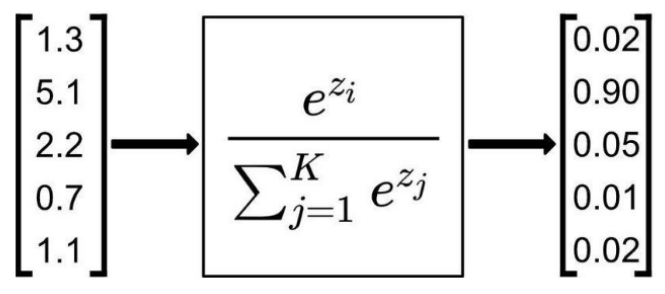
\includegraphics[width=\linewidth]{Pictures/MNLR_1.png}
    \end{subfigure}
\end{figure}
$\quad$\\[-1em]
For input $\mathbf{x}$, the score (also called \textbf{logit}) for class $c$ is $z_c=\mathbf{w}_c\cdot\mathbf{x}+b_c$. But probabilities need to be positive, so take the exponential $e^{z_c}$. But probabilities also need to sum to 1, so normalize. \\\\
The softmax function:
$$
\text{softmax}(z_i)=\frac{\text{exp}(z_i)}{\sum_{k=1}^{K}\text{exp}(z_k)}\quad\text{for }1\leq i\leq K
$$
This gives the softmax regression model:
$$
f(\mathbf{x};W,b)=\begin{bmatrix}
    P(y=1|\mathbf{x};W,b) \\
    P(y=2|\mathbf{x};W,b) \\
    \vdots \\
    P(y=K|\mathbf{x};W,b)
\end{bmatrix}
=\frac{1}{\sum_{k=1}^K \text{exp}(\mathbf{w}_{k}^{\top}\cdot\mathbf{x}+b_k)}\begin{bmatrix}
    \text{exp}(\mathbf{w}_{1}^{\top}\cdot\mathbf{x}+b_1) \\
    \text{exp}(\mathbf{w}_{2}^{\top}\cdot\mathbf{x}+b_2) \\
    \vdots \\
    \text{exp}(\mathbf{w}_K^{\top}\cdot\mathbf{x}+b_K)
\end{bmatrix}
=\text{softmax}(W\mathbf{x}+\mathbf{b})
$$
The model parameters are $W$ and $\mathbf{b}$. $W$ is a matrix with each row being the weight vector for a class. $\mathbf{b}$ is a vector of bias terms for each class.
$$
W=\begin{bmatrix}
    \mathbf{w}_1^{\top} \\
    \mathbf{w}_2^{\top} \\
    \vdots \\
    \mathbf{w}_K^{\top}
\end{bmatrix}
\quad\quad
\mathbf{b}=\begin{bmatrix}
    b_1 \\
    b_2 \\
    \vdots \\
    b_K
\end{bmatrix}
$$
Together, $\mathbf{w}_k$ and $b_k$ define the linear decision boundary for class $k$. \\\\
The cross-entropy loss is also generalized to multiple classes. Now, $\hat{y}$ is a vector of $K$ probabilities. Let $y$ be a vector of targets, setting $y_c=1$ for the true class and $y_c=0$ for all other classes.
$$
L_{\text{CE}}=-\sum_{k=1}^{K}y_k\log\hat{y}_k=-\sum_{k=1}^{K}y_k\log P(y=k|\mathbf{x})
$$
This loss corresponds to what is called the negative log-likelihood. Without the minus sign, this is once again what we want to maximize with maximum likelihood estimation.
For multinomial logistic regression, the cross-entropy loss is a function of all parameters $W,\mathbf{b}$.
\begin{align*}
    L_{\text{CE}}&=-\sum_{k=1}^{K}y_k\log\hat{y}_k \\
    &=-\log\hat{y}_c\quad\text{(where }c\text{ is the correct class)} \\
    &=-\log\hat{P}(y_c=1|\mathbf{x}) \\
    &=-\log\frac{\text{exp}(\mathbf{w}_c\cdot\mathbf{x}+b_c)}{\sum_{k=1}^{K}\text{exp}(\mathbf{w}_k\cdot\mathbf{x}+b_k)}
\end{align*}

\subsubsection{Imbalanced classes}
For binary classification, the problem is framed as mapping inputs $x$ to positive or negative labels. In a \textbf{balanced dataset}, both labels appear in \textbf{roughly equal numbers}. In an \textbf{imbalanced dataset}, \textbf{one label occurs much more often} than the other.
For example, the training set of transactions labelled fraudulent vs. legitimate can have much higher proportion of legitimate transactions.
\begin{figure}[H]
    \centering
    \begin{subfigure}{0.3\textwidth}
        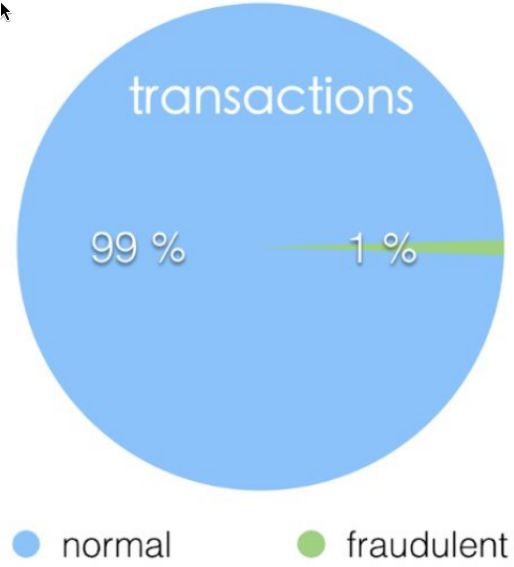
\includegraphics[width=\linewidth]{Pictures/IC_1.png}
    \end{subfigure}
\end{figure}
$\quad$\\[-1em]
The problem is, does your dataset contain enough minority class examples to train a model properly?
\begin{itemize}
    \item For mild imbalance (20\%-40\% minority) and sometimes for moderate imbalance (1\%-20\%), imbalance isn't a problem.
    \item For extreme imbalance ($<$1\% minority), the model trains almost exclusively on one label and can't learn enough about the other label.
\end{itemize}

\subsubsection{Handling imbalanced datasets}
\textbf{Downsampling majority class:} \\
Reduce the number of majority examples by randomly selecting a subset of all majority examples to train on. For example, 1:10 $\to$ downsample by $1/5$ times $\to$ 1:2.
You can perform the sampling before training starts or at the start of every epoch.
\\\\
\textbf{Upsampling minority class:} \\
Keep all majority class examples but duplicate minority class to match majority class size. For example, 1:10 $\to$ upsample by 10 times $\to$ 1:1.
\begin{warning}[Warning]
This can lead to an \textbf{increase in the risk of overfitting} since the same minority examples are repeated multiple times!
\end{warning}
\begin{note}[Upsampling/downsampling is something you have to...]
\begin{enumerate}
    \item \textbf{Apply carefully:} it can improve performance, but it is not guaranteed to. It has trade-offs e.g. overfitting with upsampling and data loss with downsampling.
    \item \textbf{Experiment with sampling ratios:} try different up/downsampling factors, e.g. 1:2, 1:3, 1:10, rather than assuming a perfectly balanaced dataset is alwasy best.
    \item \textbf{Validate on a held-out validation set:} check that performance gains generalize beyond the resampled training data.
\end{enumerate}
\end{note}

\subsection{Text classification}
Given a document $d$ and a fixed set of classes $C=\{c_1,c_2,\dots,c_K\}$, can we accurately predict the true class $c\in C$? \\\\
\textbf{Rule-based methods:}\\
These are hard-coded rules based on combinations of words or other related features. The accuracy can be high if the rules are carefully refined by the expert(s), but building and maintaining these rules is expensive. \\\\
\textbf{Machine learning methods:} \\
For machines, given data $D$ where inputs are documents and the outputs are classes, it can effectively learn a classifier $h:X\to Y$.

\subsubsection{Bag-of-words}
In a bag-of-words approach, we represent documents with word counts ignoring order.
\begin{enumerate}
    \item Tokenize text into words and assign an integer ID to each unique word in the training dataset, called the vocabulary.
    \item Count the word occurences in each document.
    \item Each document becomes a vector of indexed counts.
\end{enumerate}
\begin{figure}[H]
    \centering
    \begin{subfigure}{0.7\textwidth}
        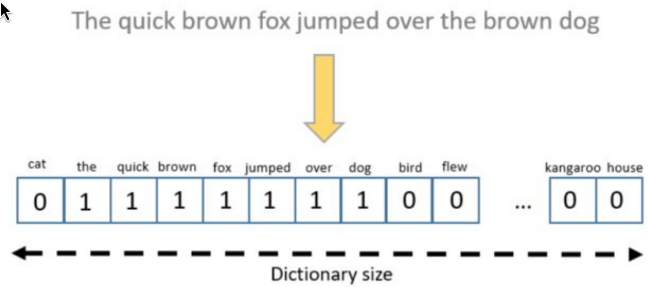
\includegraphics[width=\linewidth]{Pictures/BoW_1.png}
    \end{subfigure}
\end{figure}
$\quad$\\[-1em]
Word counts can be informative features for classification tasks. In logistic regression, each feature (word) will have a weight parameter $w_i$, which encodes its influence on predictions.
\begin{figure}[H]
    \centering
    \begin{subfigure}{0.7\textwidth}
        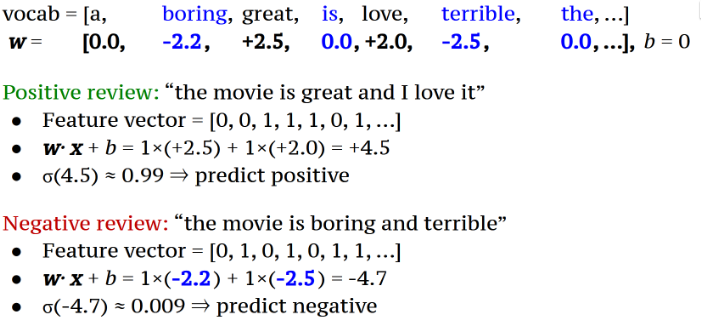
\includegraphics[width=\linewidth]{Pictures/BoW_2.png}
    \end{subfigure}
\end{figure}
$\quad$\\[-1em]
Most words never appear in a given document.
\begin{itemize}
    \item Vocabulary can be very large (e.g. 100k words).
    \item Each document uses only a small fraction (100-1000 words), so most vectors are mostly zero ($>$99\%).
    \item It is common to use sparse data structures for storage and efficiency.
\end{itemize}
\begin{note}[Design choices affect what ends up in your vocabulary.]
\begin{itemize}
    \item \textbf{Text preprocessing/cleaning:} lowercase words, remove puncuation or number if not useful.
    \item \textbf{Tokenization:} the simple, straightforward approach is to split on whitespace characters. There are more sophisicated tokenizers available.
    \item \textbf{Vocabulary size control:} \textit{(based on training data frequencies!)}
    \begin{itemize}
        \item Keep only top $N$ frequent words (tune $N$).
        \item Don't include rare words (occurs less than some frequency threshold).
    \end{itemize}
    \begin{warning}[Tradeoff]
        A bigger vocabulary could produce better features, but might result in slower training!
    \end{warning}
\end{itemize}
\end{note}

\subsubsection{Binary presence}
Another option is to simplify bag-of-words to presence/absence of words.
\begin{itemize}
    \item Feature = 1 if word appears, 0 otherwise.
    \item Ignores frequency of word within document.
    \item Useful when word presence is more informative than counts.
\end{itemize}

\subsubsection{TF-IDF}
The problem is that raw words counts are misleading because common words like "the" or "is" appear everywhere but add zero meaning. Truly informative words (e.g "remarkable", "special", "uninspiring") are rare and give a document its unique identity.
We can use TF-IDF (term frequency - inverse document frequency) to scale down frequent, generic words and scale up rare, highly descriptive words to surface the most meaningful features. \\\\
\textbf{TF (term frequency):} number of times term $t$ appears in document $d$ divided by total number of terms in document $d$. \\\\
\textbf{IDF (inverse document frequency):}\\
\begin{itemize}
    \item $\text{idf}(t)=\log(N/\text{df}(t))$, where
    \item $N$ is the number of documents in the training set, $\text{df}(t)$ id the number of documents containing term $t$.
    \item $\text{idf}(t)$ is low if term $t$ is common and high when term $t$ is rare.
\end{itemize}
\textbf{TF-IDF:} $\text{tf}\times\text{idf}$
\begin{note}[Extra]
Usually the TF-IDF vector is L2-normalized. Reminder on L2-normalization:
$$
x_{ij}^{\text{new}}=\frac{x_{ij}}{\sqrt{\sum_{i=1}x_{ij}^2}}
$$
\end{note}

\subsubsection{Example 1}
Suppose we have 100 documents of 200 words each. The term "the" appears 20 times in document $d$ and in 90 documents overall.
\begin{itemize}
    \item $\text{tf}(\text{"the"},d)=20/200=0.1$
    \item $\text{idf}(\text{"the"})=\log(100/90)=0.046$
    \item $\text{tf-idf}(\text{"the"},d)=0.1\times 0.046=0.0046$
\end{itemize}

\subsubsection{Example 2}
Suppose we have 100 documents of 200 words each. The term "happy" appears 5 times in document $d$ and in 5 documents overall.
\begin{itemize}
    \item $\text{tf}(\text{"happy"},d)=5/200=0.025$
    \item $\text{idf}(\text{"happy"})=\log(100/5)\approx 3$
    \item $\text{tf-idf}(\text{"happy"},d)=0.025\times 3=0.075$
\end{itemize}

\subsection{Regularization}
\subsubsection{Interpreting logistic regression}
After training, learned weights capture how each feature contributes to model predictions, giving us insight into what the model has learned.
\begin{figure}[H]
    \centering
    \begin{subfigure}{0.8\textwidth}
        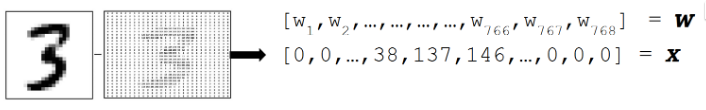
\includegraphics[width=\linewidth]{Pictures/R_1.png}
    \end{subfigure}
\end{figure}
$\quad$\\[-1em]
The magnitude of a weight $|w_i|$ reflects how strongly the associated feature influences the final predictions. Larger values have a stronger effect. The sign of $w_i$ shows the direction of influence. Positive weights push the prediction towards class 1, while negative weights push the prediction towards class 0.
\subsubsection{Overfitting}
\begin{definition}[Overfitting]
Overfitting is when your model is fitting the details of the training data so closely that the model doesn't generalize well to the test set. 
This happens when the model is over-parameterized. In other words, it has more parameters than required to model the data.
The model is "too powerful", so it memorizes the training data. It predicts training data perfectly, but cannot generalize to new data.
\end{definition}
\begin{figure}[H]
    \centering
    \begin{subfigure}{0.8\textwidth}
        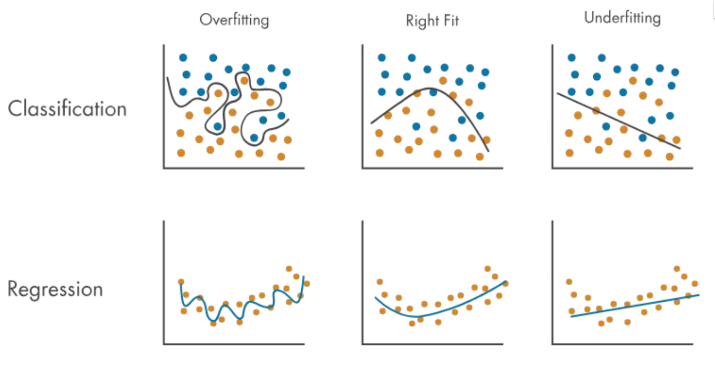
\includegraphics[width=\linewidth]{Pictures/R_2.png}
    \end{subfigure}
\end{figure}
$\quad$\\[-1em]
How can overfitting happen for logistic regression?
\begin{itemize}
    \item The weight $w_i$ is learned such that $w_ix_i$ contributes to improved accuracy.
    \item If a feature $x_i$ occurs only in one class in the training data, the model could learn very high weight $w_i$ and perfectly predict $y$.
    \item The model might be over-relying on the presence of this feature, due to a peculiar property of the training data.
    \item The model will fail to generalize to a test set without this feature.
\end{itemize}
\begin{note}[Tracking performance]
\textbf{High training accuracy, but low validation accuracy OR low training loss, but high validation loss.}
\begin{itemize}
    \item That's why it's important to track validation perfroamcne during training!
    \item If you only track training performance, this tells you nothing about how your model will generalize.
\end{itemize}
\end{note}
Potential causes of overfitting:
\begin{itemize}
    \item \textbf{Wrong model for task:} model complexity exceeds available data.
    \item \textbf{Training data too small:} model will memorize rather than generalize.
    \item \textbf{Low-quality training data:} too much noise, which the model learns as if it is signal noise.
    \item \textbf{Too many training epochs:} eventually model fits training set too closely.
\end{itemize}

\subsubsection{Early stopping}
\begin{definition}[Early stopping]
Stop training when the performance on held-out dataset stops improving to avoid overfitting.
\end{definition}
$\quad$\\[-1em]
Validation performance usually improve before degrading with overfitting. After this, improving training data fit comes at expense of generalization. Continually monitor performance on validation dataset and stop training where validation accuracy peaks.

\subsubsection{Regularization}
Add a regularization term $R(\theta)$ to the objective function.
$$
\hat{\theta}=\underset{\theta}{\text{argmax}}\Big[\sum_{i=1}^{B}\log P(y_i|\mathbf{x}_i;\theta)-\alpha R(\theta)\Big]
$$
Choose $R(\theta)$ to penelize large parameters $\theta$. Loss favors predicting data less well with small $\theta$ than predicting data well with big $\theta$. More formally, we force optimization to balance maximizing the log-likelihood while minimizing weight magnitudes.

\subsubsection{L2 Regularization}
The regularization term is the sum of the squares of the weights. The L2 norm $||\theta||_2$ is the Euclidean distance of $\theta$ to the origin.
$$
R(\theta)=||\theta||_2^2=\sum_{i=1}^{n}\theta_{i}^2
$$
The L2 regularized log-likelihood:
$$
\hat{\theta}=\underset{\theta}{\text{argmax}}\Big[\sum_{i=1}^{B}\log P(y_i|\mathbf{x}_i;\theta)-\alpha\sum_{i=1}^{n}\theta_{n}^2\Big]
$$
This is equivalent to minimizing the cross-entropy loss plus the L2 norm.
$$
\hat{\theta}=\underset{\theta}{\text{argmax}}\Big[\frac{1}{B}\sum_{i=1}^{B}L_{\text{CE}}(\hat{y}_i,y_i)+\alpha\sum_{i=1}^n\theta_{n}^2\Big]
$$

\subsubsection{L1 Regularization}
The regularization term is the sum of the absolute values of the weights. The L1 norm $||\theta||$ is the Euclidean distance of $\theta$ to the origin.
$$
R(\theta)=||\theta||_1=\sum_{i=1}^{n}|\theta_{i}|
$$
The L1 regularized log-likelihood:
$$
\hat{\theta}=\underset{\theta}{\text{argmax}}\Big[\sum_{i=1}^{B}\log P(y_i|\mathbf{x}_i;\theta)-\alpha\sum_{i=1}^{n}|\theta_{n}|\Big]
$$
This is equivalent to minimizing the cross-entropy loss plus the L1 norm.
$$
\hat{\theta}=\underset{\theta}{\text{argmax}}\Big[\frac{1}{B}\sum_{i=1}^{B}L_{\text{CE}}(\hat{y}_i,y_i)+\alpha\sum_{i=1}^n|\theta_{n}|\Big]
$$

\subsubsection{Regularization (continued)}
L2 regularization produces weight vectors with many small weights:
$$
[0.05,-0.01,0.01,-0.005,0.1,\dots]
$$
L1 regularization tends to produce sparse solutions with some larger weights but many more weights set to zero.
$$
[1.1,0.0,-2.5,0.0,0.0,\dots]
$$
$$
\hat{\theta}=\underset{\theta}{\text{argmax}}\Big[\sum_{i=1}^{B}\log P(y_i|\mathbf{x}_i;\theta)-\alpha R(\theta)\Big]
$$
\begin{itemize}
    \item $\alpha$ is a hyperparameter that controls the strength of regularization.
    \item During training, the model is baised towards smaller parameter values, which prevent over-reliance on certain features.
    \item These features could be unique to the training data, so not relying on them can reduce overfitting.
\end{itemize}

\subsection{Naive Bayes}
\subsubsection{Generative vs. discriminative classifiers}
\textbf{Generative models} learn the distribution of individual classes $P(x|y)$.
Model how data is generated. Given a new example to classify, based on generation assumption, which category is most likely to generate this data?
\\\\
\textbf{Discriminative models} learn the boundaries between classes $P(y|x)$. Model decision boundary between classes rather than underlying distribution of each class. Learns defining differences between classes and classifies examples based on these differences.
\\\\
\textbf{Discriminative classifier:} estimate the posterior $P(y|x)$ directly. This is what logistic regression computes.
$$
y=\underset{y\in C}{\text{argmax}}\hspace{2pt}\overbrace{P(y|x)}^{\text{posterior}}
$$
\begin{figure}[H]
    \centering
    \begin{subfigure}{0.6\textwidth}
        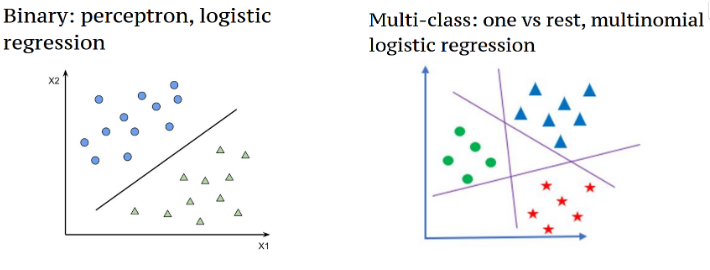
\includegraphics[width=\linewidth]{Pictures/NB_1.png}
    \end{subfigure}
\end{figure}
$\quad$\\[-1em]
\textbf{Generative classifier:} estimate likelihood $P(x|y)$ and apply Bayes' rule.
$$
y=\underset{y\in C}{\text{argmax}}\overbrace{P(x|y)}^{\text{likelihood}}\overbrace{P(y)}^{\text{prior}}
$$

\subsubsection{Independence}
\begin{definition}[Independence of events]
Two events $X$ and $Y$ are independent when knowing one tells you nothing about the other. In other words, learning $Y$ does not change the probability of $X$.
\end{definition}
$\quad$\\[-1em]
That is,
$$
P(X|Y)=P(X)\iff P(Y|X)=P(Y)
$$
If two events are independent, then te following holds:
$$
P(X,Y)=P(X)P(Y)
$$

\subsubsection{Bayes' rule}
Two ways to factor a join distribution over two variables:
$$
P(x,y)=\frac{P(y)P(x|y)}{P(x)}
$$
Dividing, we get Bayes' rule:
$$
\boxed{P(y|x)=\frac{P(y)P(x|y)}{P(x)}}
$$
where:
\begin{itemize}
    \item $P(y|x)$ is the \textbf{posterior probability}.
    \item $P(y)$ is the \textbf{prior}.
    \item $P(x)$ is the \textbf{evidence}.
    \item $P(x|y)$ is the \textbf{likelihood}.
\end{itemize}

\subsubsection{Naive Bayes classifier}
Naive Bayes is a simple classification method based on Bayes' rule. For a document $d$, Bayes' rule can be used to calculate $P(c|d)$ for every output class $C=\{c_1,c_2,\dots,c_K\}$.
$$
P(c|d)=\frac{P(c)P(d|c)}{P(d)}
$$
To obtain a prediction, find the class for which $P(c|d)$ is highest:
$$
c_{\text{MAP}}=\underset{c\in C}{\text{argmax}}\hspace{2pt}P(c|d)
$$
MAP stand for "maximum a posteriori", or in other words most likely class.
\begin{note_special}[Derivation]
\begin{align*}
    c_{\text{MAP}}&=\underset{c\in C}{\text{argmax}}\hspace{2pt}P(c|d) \\
    &= \underset{c\in C}{\text{argmax}}\hspace{2pt}\frac{P(c)P(d|c)}{P(d)}\quad\text{(Bayes' rule)} \\
    &=\underset{c\in C}{\text{argmax}}\hspace{2pt}P(d|c)P(c)\quad\text{(Drop denominator, argmax unaffected)} \\
    &=\underset{c\in C}{\text{argmax}}\hspace{2pt}P(x_1,x_2,\dots,x_n|c)P(c)\quad\text{(Represent document as features)}
\end{align*}
\end{note_special}
$\quad$\\[-1em]
How can we estimate these probabilities? The simple solution is to just count how often each class occurs and then normalize. 
\\\\
\textbf{Bag-of-words assumption:} Assume word positions doesn't matter. \\\\
\textbf{Conditional independence:} Assume the feature probabilities $P(x_i|c_i)$ are independent given the class $c$:
$$
P(x_1,x_2,\dots,x_n|c)=P(x_1|c)\times P(x_2|c)\times\cdots\times P(x_n|c)
$$
We can estimate these probabilities:
$$
\hat{P}(w_i|c_j)=\frac{\text{count}(w_i,c_j)}{\sum_{w\in V}\text{count}(w,c_j)}
$$
In other words, the relative frequency of $w_i$ within class $c_j$. We can estimate $P(c)$ in the following way:
$$
\hat{P}(c_j)=\frac{N_{cj}}{N_\text{total}}
$$
where $N_{cj}$ is the number of training examples in class $c_j$ and $N_{\text{total}}$ is the total number of training examples. Given our assumption, we can rewrite the prediction for Naive Bayes as:
\begin{align*}
    c_{\text{NB}}&=\underset{c\in C}{\text{argmax}}\hspace{2pt}P(c_j)\prod_{x\in X}P(x|c) \\
    &= \underset{c\in C}{\text{argmax}}\hspace{2pt}P(c_j)\prod_{i\in\text{positions}}P(x_i|c_j)
\end{align*}
where $i\in\text{positions}$ goes through all words in the document. While this is great, it comes with an implementation problem. Multiplying lots of probabilities can results in floating-point underflow. To combat this, simply use log probabilities!
\begin{align*}
    c_{\text{NB}}&=\underset{c\in C}{\text{argmax}}\hspace{2pt}P(c_j)\prod_{i\in\text{positions}}P(x_i|c_j) \\
    &=\underset{c\in C}{\text{argmax}}\Big[\log P(c_j)+\sum_{i\in\text{positions}}\log P(x_i|c_j)\Big]
\end{align*}

\subsubsection{Naive Bayes classifier: learning}
The problem with maximum likelihood is the zero counts. What is we have seen no training documents with the word "fantastic" and labelled as "positive"? If any of the probability terms are 0, the whole probability score will be 0.
\\\\
\textbf{Solution: Laplace (add-1) smoothing} \\
Add 1 to the count of each $(w,c)$:
$$
\hat{P}(w_i|c)=\frac{\text{count}(w_i,c)+1}{\sum_{w\in V}\text{count}(w,c)+|V|}
$$
where $|V|$ is the size of the vocabulary. Unknown words get a tiny probability. Frequent words still dominate.
\\\\
\textbf{Solution: Additive smoothing}\\
Add $\alpha$ to the count of each $(w,c)$:
$$
\hat{P}(w_i|c)=\frac{\text{count}(w_i,c)+\alpha}{\sum_{w\in V}\text{count}(w,c)+\alpha|V|}
$$
Here, $\alpha$ is the smoothing parameter. It controls how much probability mass you give to unseen events. If $\alpha=1$, that's classic Laplace smoothing.
\\\\
\textbf{Training algorithm:}
\begin{enumerate}
    \item From training corpus, extract the vocabulary.
    \item Calculate $P(c_j)$ terms.
    \item Calculate $P(w_k|c_j)$ terms.
\end{enumerate}
\begin{note}[Extra]
What about unknown words that appear in the test data but not in the training data? It doesn't necessarily help. Knowing which class has more unkown words is not generally helpful.
\end{note}

\subsubsection{Example}
\begin{figure}[H]
    \centering
    \begin{subfigure}{0.6\textwidth}
        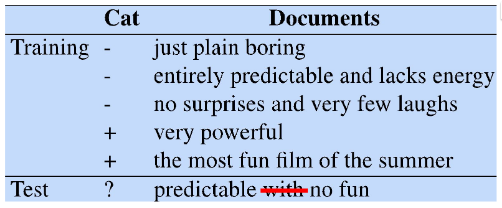
\includegraphics[width=\linewidth]{Pictures/NB_2.png}
    \end{subfigure}
\end{figure}
$\quad$\\[-1em]
\begin{enumerate}
    \item Create vocabulary: 20 unique words in training data.
    \item Calculate the priors from training: $\hat{P}(c_j)=N_{cj}/N_{\text{total}}$
$$
P(-)=3/5\quad\quad P(+)=2/5
$$
    \item Calculate likelihoods from training (Laplace smoothing). Here we have 14 tokens in negative docs and 9 in positive docs.
\begin{align*}
    P(\text{"predictable"}|-)&=\frac{1+1}{14+20} & P(\text{"predictable"}|+)&=\frac{0+1}{9+20} \\
    P(\text{"no"}|-)&=\frac{1+1}{14+20} & P(\text{"no"}|+)&=\frac{0+1}{9+20} \\
    P(\text{"fun"}|-)&=\frac{0+1}{14+20} & P(\text{"fun"}|+)&=\frac{1+1}{9+20}
\end{align*}    
    \item Scoring the test example:
\begin{align*}
    P(-)P(\text{"predicatble"}|-)P(\text{"no"}|-)P(\text{"fun"}|-)&=0.6\times\frac{4}{32^2}=6.1\times 10^{-5} \\
    P(+)P(\text{"predicatble"}|+)P(\text{"no"}|+)P(\text{"fun"}|+)&=0.4\times\frac{2}{29^2}=3.2\times 10^{-5}
\end{align*}
\end{enumerate}

\subsubsection{Binary Naive Bayes}
For tasks like sentiment analysis, word occurence can be more important than word frequency. For example, the occurence of the word "fantastic" tells us a lot. The fact that it occurs 5 times may not tell us much more.
Binary Naive Bayes is a variant of Naive Bayes:
\begin{itemize}
    \item Clip our word counts at 1 for each document.
    \item Can implement by removing duplicates in each document and executing Naive Bayes algorithm as before.
\end{itemize}
\begin{figure}[H]
    \centering
    \begin{subfigure}{0.7\textwidth}
        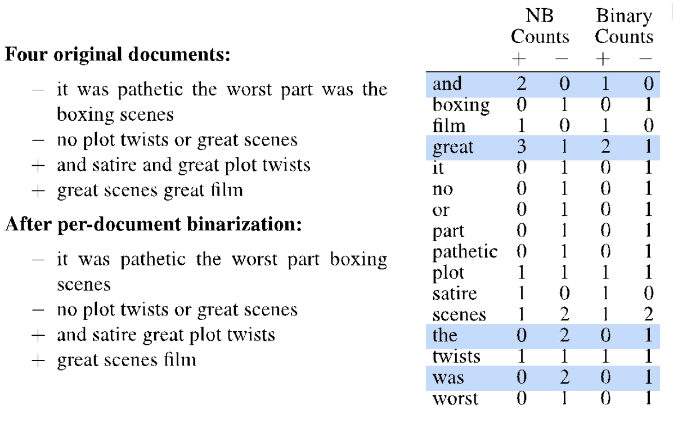
\includegraphics[width=\linewidth]{Pictures/NB_3.png}
    \end{subfigure}
\end{figure}

\section{Artificial Neural Networks}
\subsection{Neural networks}
Artificial neural networks (ANNS) consist of artificial neurons, much like brain cells, and are connected to each other via synapses.
The artificial neurons pass signals (real numbers) between each other. Given some input, we would like to make a decision.
Typically, we use non-linear activation functions for each neuron.

\begin{figure}[H]
    \centering
    \begin{subfigure}{0.5\textwidth}
        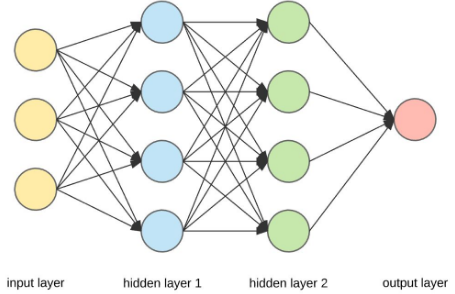
\includegraphics[width=\linewidth]{Pictures/ANN_1.png}
    \end{subfigure}
\end{figure}

\subsubsection{Neural network architecture}
A neural network consists of:
\begin{itemize}
    \item An input layer
    \item Hidden layer(s)
    \item An output layer
\end{itemize}
Each unit layer computes a value based on the linear combination of values of units to that point into it.
What happens if you add more hidden layers? Increase the \textit{depth} of the neural network.

\subsection{Feedforward propagation formulation}
\subsubsection{Activation functions}
\begin{definition}[Activation function]
The mathematical equation inside a neuron that determines the neuron's output.
\end{definition}
$\quad$\\[-1em]
What is the role of the activation function? It is used to introduce non-linearity into the neural network.
How do they even work? Every neuron has two stages:
\begin{enumerate}
    \item \textbf{Weighted sum:} The neuron receives inputs from the previous layer.
    Each input is multiplied bt a weight. These are all summed up, and a bias term is added.
    This results in a single number $z$.
    \item \textbf{Activation:} This number $z$ is then passed through the activation function, say $f(z)$,
    to produce the neuron's final output $y$. This output is then sent as an input to the neurons
    in the next layer.
\end{enumerate}
\begin{figure}[H]
    \centering
    \begin{subfigure}{0.8\textwidth}
        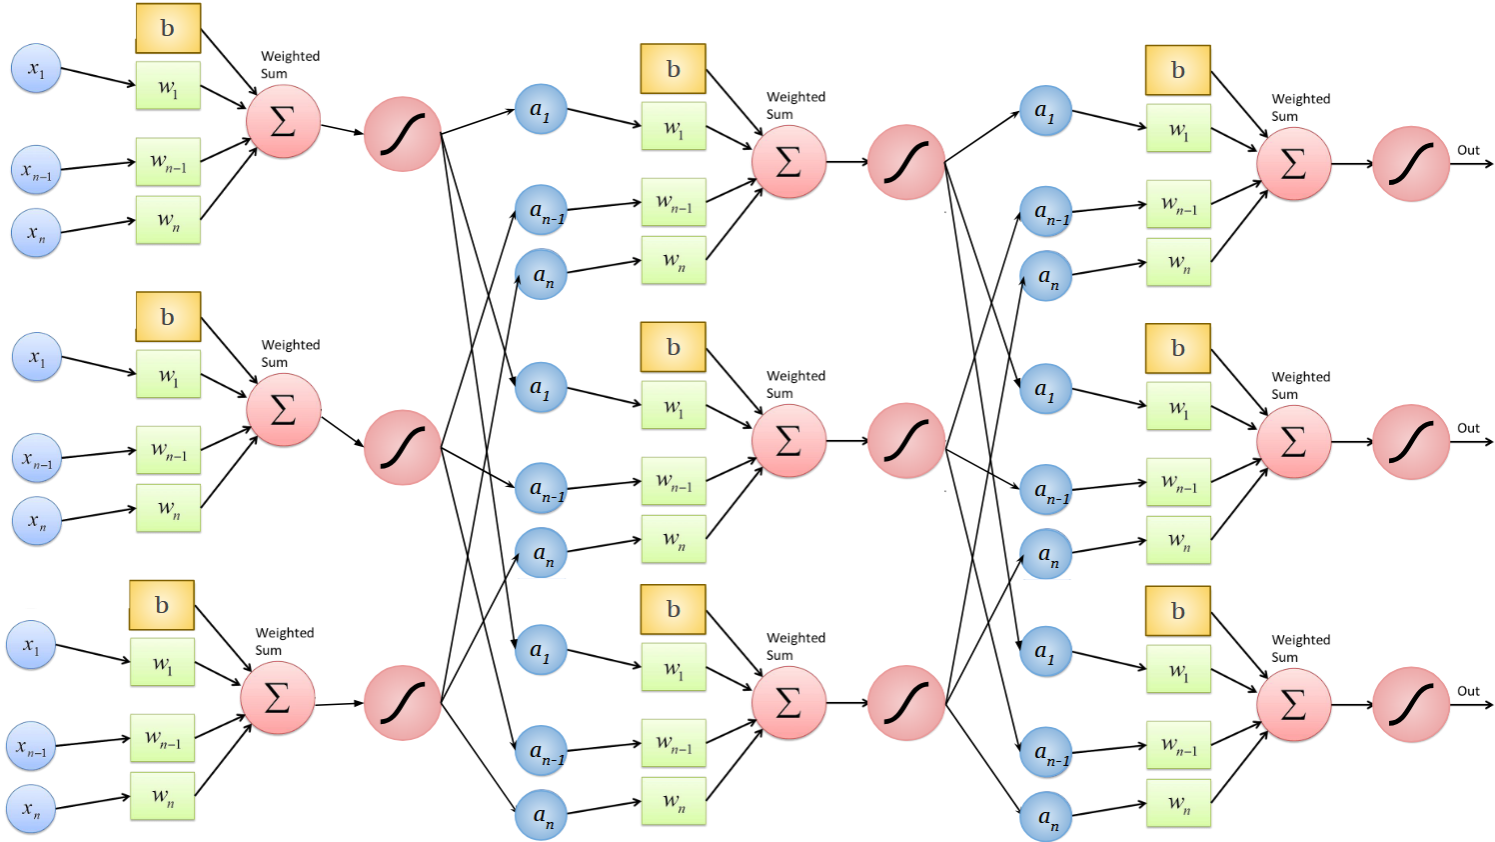
\includegraphics[width=\linewidth]{Pictures/ANN_2.png}
    \end{subfigure}
\end{figure}
\begin{note}[Note]
Every layer in a neural network has its own activation function.
\end{note}

\subsubsection{Network structure}
\begin{figure}[H]
    \centering
    \begin{subfigure}{0.8\textwidth}
        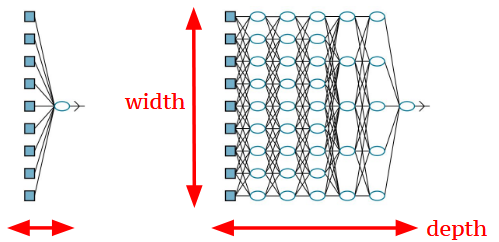
\includegraphics[width=\linewidth]{Pictures/ANN_3.png}
    \end{subfigure}
\end{figure}
$\quad$\\[-1em]
A \textbf{feedforward network} has connections going in one direction.
Logistic regression can be viewed as ashallow (1-layer) neural network.
Let each connection (line) represent a weight multiplication with the preceding unit output, and
all incoming lines represent a weighted sum. Each unit computes: $a_j=g_j(\mathbf{w}_{j}^{\top}\mathbf{x}+b_j)$
\begin{itemize}
    \item A weighted sum of its weights with the output of the previous layer.
    \item Passes that through an activation function $g$.
\end{itemize}

\subsubsection{Non-linearity}
Each unit $j$ has a \textbf{nonlinear} activation function $g_j$ through which the weighted sum is passed.
Without nonlinearity, any composition of units would still represent a linear function.
The nonlinearity allows sufficiently large networks of units to approximate arbitrary functions.
Unlike linear regression, perceptrons, and logistic regression neural networks can model non-linear functions for regression or classification.
\begin{figure}[H]
    \centering
    \begin{subfigure}{0.6\textwidth}
        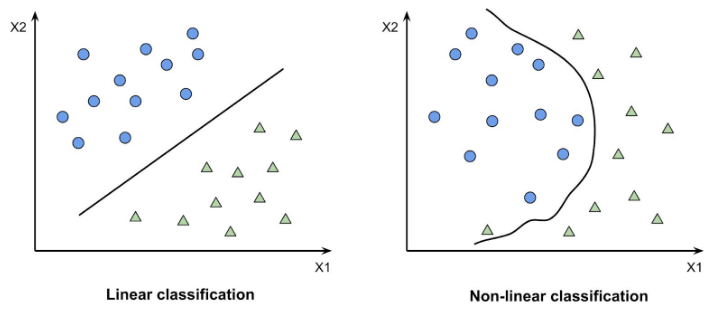
\includegraphics[width=\linewidth]{Pictures/ANN_4.png}
    \end{subfigure}
\end{figure}
\begin{note_special}[Theorem: Universal approximation theorem]
A network with just 2 layers, the first non-linear and the second linear, can approximate any continuous function to arbitrary degree of accuracy, including non-linear function.
\begin{figure}[H]
    \centering
    \begin{subfigure}{0.7\textwidth}
        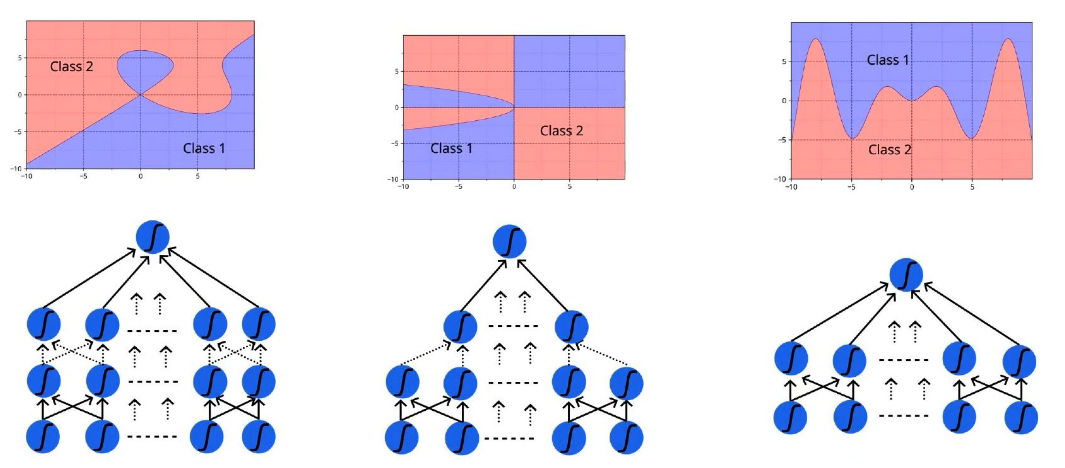
\includegraphics[width=\linewidth]{Pictures/ANN_5.png}
    \end{subfigure}
\end{figure}
\end{note_special}

\subsection{Activation functions}
All of the following are monotonically non-decreasing (positive gradients).
The choice of activation function is a modelling decision.
It depends on factors like the task, the type of neural network, etc.
\subsubsection{Sigmoid}
\begin{minipage}{0.5\textwidth}
$$
\sigma(x)=\frac{1}{1+e^{-x}}
$$
As seen with logistic regression.
\end{minipage}
\begin{minipage}{0.5\textwidth}
\begin{figure}[H]
    \centering
    \begin{subfigure}{0.6\textwidth}
        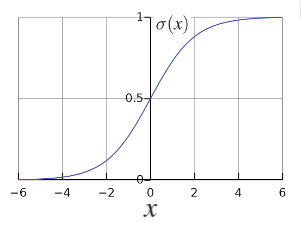
\includegraphics[width=\linewidth]{Pictures/ANN_6.png}
    \end{subfigure}
\end{figure} 
\end{minipage}

\subsubsection{ReLU}
\begin{minipage}{0.5\textwidth}
$$
\text{ReLU}(x)=\max(0,x)
$$
Non-linear function (gradient is not constant) but acts linear for part of the domain ($>$0).
This is a very commonly used activation function.
\end{minipage}
\begin{minipage}{0.5\textwidth}
\begin{figure}[H]
    \centering
    \begin{subfigure}{0.6\textwidth}
        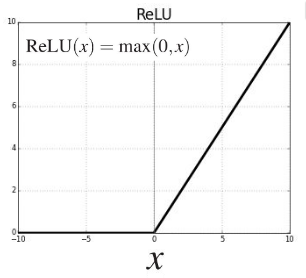
\includegraphics[width=\linewidth]{Pictures/ANN_7.png}
    \end{subfigure}
\end{figure} 
\end{minipage}

\subsubsection{Softplus}
\begin{minipage}{0.5\textwidth}
$$
\text{softplus}(x)=\log(1+e^{x})
$$
The smooth version of ReLU function.
\end{minipage}
\begin{minipage}{0.5\textwidth}
\begin{figure}[H]
    \centering
    \begin{subfigure}{0.6\textwidth}
        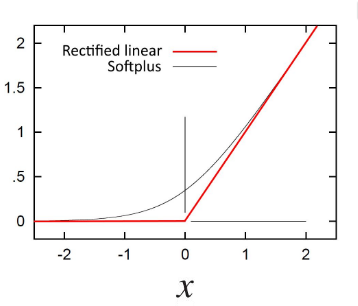
\includegraphics[width=\linewidth]{Pictures/ANN_8.png}
    \end{subfigure}
\end{figure} 
\end{minipage}

\subsubsection{Tanh}
\begin{minipage}{0.5\textwidth}
$$
\tanh(x)=\frac{e^{2x}-1}{e^{2x}+1}
$$
Range of $\tanh$ is $[-1,1]$. It is the scaled and shifted version of the sigmoid,
$$
\tanh(x)=2\sigma(2x)-1
$$
\end{minipage}
\begin{minipage}{0.5\textwidth}
\begin{figure}[H]
    \centering
    \begin{subfigure}{0.6\textwidth}
        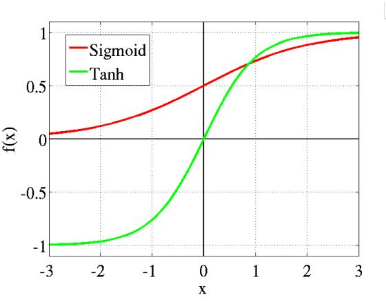
\includegraphics[width=\linewidth]{Pictures/ANN_9.png}
    \end{subfigure}
\end{figure} 
\end{minipage}

\subsection{Deep neural networks}
\begin{definition}[Deep neural networks]
A deep neural network has
\begin{itemize}
    \item An input layer: input vector $x$.
    \item Hidden layer(s): itermediate representations.
    \item An output layer: predicting output values for $y$ e.g. probabilities.
\end{itemize}
\end{definition}
\begin{figure}[H]
    \centering
    \begin{subfigure}{0.6\textwidth}
        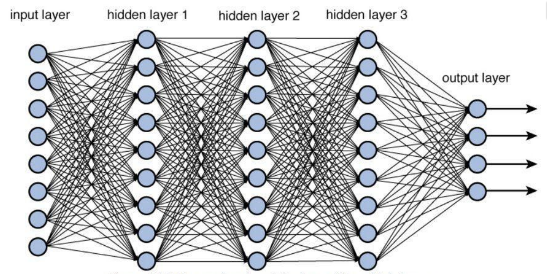
\includegraphics[width=\linewidth]{Pictures/ANN_10.png}
    \end{subfigure}
\end{figure} 
In a \textbf{fully connected} network, every node in each layer is connected to every node in the next layer.
A unit calculates the weighted sum of the inputs from predecessor nodes and plies some activation function to it.
Let $a_j$ denote the output of unit $j$, let $w_{i,j}$ be the weight attaching unit $i$ to unit $j$.
Let $b_j$ be the bias and $g_j$ the activation function of unit $j$. Then
\begin{align*}
    a_j&=g_j\Big(\sum_i w_{i,j}a_i+b_j\Big) \\
    &=g_j(\mathbf{w}_j^{\top}\mathbf{x}+b_j)
\end{align*}
where $\mathbf{w}_j$ is the vector of weights into unit $j$ and $\mathbf{x}$ is the vector of inputs for unit $i$.
\begin{figure}[H]
    \centering
    \begin{subfigure}{0.5\textwidth}
        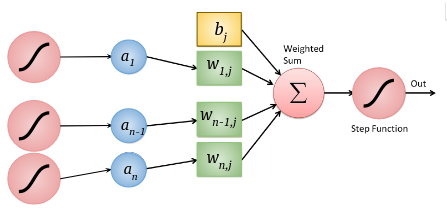
\includegraphics[width=\linewidth]{Pictures/ANN_11.png}
    \end{subfigure}
\end{figure}
$\quad$\\[-1em]
This describes the operation of a single unit in vector form.
We can describe entire layers and networks in matrix form. 

\subsubsection{Matrix notation}
\begin{minipage}{0.5\textwidth}
\begin{figure}[H]
    \centering
    \begin{subfigure}{0.7\textwidth}
        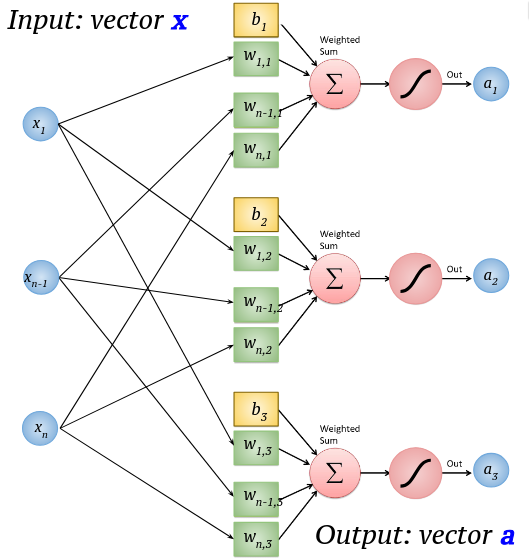
\includegraphics[width=\linewidth]{Pictures/ANN_12.png}
    \end{subfigure}
\end{figure} 
\end{minipage}
\begin{minipage}{0.5\textwidth}
Each unit a weight vector $\mathbf{w}_i$ and a bias term $b_i$. Combine the weight vectors into a matrix $W$,
and the biases into a vector $\mathbf{b}$:
$$
W=\begin{bmatrix}
\leftarrow w_1^{\top} \rightarrow \\
\leftarrow w_2^{\top} \rightarrow \\
\leftarrow w_3^{\top} \rightarrow
\end{bmatrix}
\quad
\mathbf{b}=\begin{bmatrix}
b_1 \\
b_2 \\
b_3
\end{bmatrix}
$$
$W^{(i)}$ is the weight matrix of the $i$-th layer, each row corresponding to the weight vector of a unit.
$\mathbf{b}^{(i)}$ is the vector of biases of the $i$-th layer.
Then $\mathbf{a}=g(W\mathbf{x}+\mathbf{b})$.
\end{minipage}
\begin{minipage}{0.5\textwidth}
\begin{figure}[H]
    \centering
    \begin{subfigure}{0.7\textwidth}
        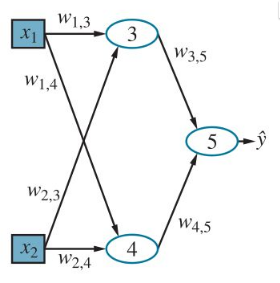
\includegraphics[width=\linewidth]{Pictures/ANN_13.png}
    \end{subfigure}
\end{figure} 
\end{minipage}
\begin{minipage}{0.5\textwidth}
\begin{align*}
\hat{y}&=g_5(\text{in}_5)=g_5(w_{0,5}+w_{3,5}a_3+w_{4,5}a_4) \\
&=g_5(w_{0,5}+w_{3,5}g_3(\text{in}_3)+w_{4,5}g_4(\text{in}_4)) \\
&=g_5(w_{0,5}+w_{3,5}g_3(w_{0,3}+w_{1,3}x_1+w_{2,3}x_2) \\
&+w_{4,5}g_4(w_{0,4}+w_{1,4}x_1+w_{2,4}x_2))
\end{align*}
\end{minipage}
Here, 
\begin{itemize}
    \item $W^{(1)}$ is the weights of the first layer ($w_{1,3}$, $w_{1,4}$, etc)
    \item $W^{(2)}$ is the weights of the second layer ($w_{3,5}$, etc)
    \item $g^{(1)}$ and $g^{(2)}$ are the activation functions in the first and second layer, respectively.
\end{itemize}
Then the entire network can be written as 
$$
h_{W}(\mathbf{x})=g^{(2)}\big(W^{(2)}g^{(1)}(W^{(1)}\mathbf{x})\big)
$$
If we include the biases as well
$$
\boxed{h_{W,\mathbf{b}}(\mathbf{x})=g^{(2)}\big(W^{(2)}g^{(1)}(W^{(1)}\mathbf{x}+\mathbf{b}^{(1)})+\mathbf{b}^{(2)}\big)}
$$

\subsection{Cost function}
Also known as the loss function. The initialization of weight and bias values are initially random.
The purpose of the loss function is to grade the performance of the neural network. High loss signifies large error and poor performance.
A low loss indicates that the network's predictions are close to the actual values.

\subsection{Optimization}
Let the loss function be parameterized by parameters $\theta=(W^{(i)},\mathbf{b}^{(i)})$ for $i=1,\dots,L$ where $L$ is the number of layers.
Let's represent our prediction $\hat{y}$ as $f(\mathbf{x};\theta)$. 
We want to find weights that minimize the loss, averaged over all examples in our training set $\{(\mathbf{x}_1,y_1),(\mathbf{x}_2,y_2),\dots,(\mathbf{x}_m,y_m)\}$
$$
\hat{\theta}=\underset{\theta}{\text{argmax}}\hspace{2px}\frac{1}{m}\sum_{i=1}^{m}L_{\text{CE}}(f(\mathbf{x}^{(i)};\theta),y^{(i)})
$$
There is no closed form solution, so we have to use general purpose techniques for mathemetical optimization.
For neural networks:
\begin{itemize}
    \item The loss function is non-convex (has more than one minimum).
    \item Gradient descent from any point is guaranteed to find a local minimum, but not necessarily the global minimum.
    \item Gradient descent still works in practice. It finds a minima that leads to good performance.
\end{itemize}
\begin{figure}[H]
    \centering
    \begin{subfigure}{0.6\textwidth}
        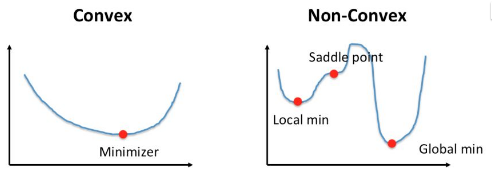
\includegraphics[width=\linewidth]{Pictures/ANN_14.png}
    \end{subfigure}
\end{figure} 
$\quad$\\[-1em]
For $n$-dimensional gradients:
\begin{itemize}
    \item The gradient of a function of many variables is a vector pointing in the direction of the greatest increase in a function.
    \item To determine the step size, the value of the gradient is weighted by a learning rate $\eta$.
\end{itemize}
$$
w^{t+1}=w^t-\eta\frac{d}{dw}L(f(x;w),y)
$$
The final equation for updating parameters $\theta$ based on the gradient is
$$
\theta^{t+1}=\theta^{t}-\eta\nabla_{\theta}L(f(\mathbf{x};\theta),y)
$$

\subsection{Back-propagation}
\subsubsection{A quick review of the chain rule}
The chain rule tells us how to differentiate composite functions. A function is composite if you can write it as $f(g(x))$.
In other words, it is a function of a function. The chain rule allows us to write the derivative of the composite function in terms of the derivatives of $g(x)$ and $f(x)$.
$$
\boxed{\frac{d}{dx}\big[f(g(x))\big]=f'(g(x))\cdot g'(x)}
$$
We can also write it in Leibniz's notation:
$$
f(x)=u(v(x)) \to \frac{df}{dx}=\frac{du}{dx}\cdot \frac{dv}{dx}
$$
$$
f(u(v(w(x)))) \to \frac{df}{dx}=\frac{du}{dx}\cdot\frac{dv}{dx}\cdot\frac{dw}{dx}
$$

\subsubsection{What is back-propagation?}
We have looked at forward-propagation. Now we move to back-propagation.
Back-propagation allows a neural network to learn from its mistakes. Its main job is to efficiently calculate how much every signle weight and bias in the network contributed to the final error.
A clever and efficient way to solve this problem is to use the chain rule from calculus.
A neural network is a series of composite functions. Apply the chain rule to find the derivative of the loss with respect to a specific parameter (e.g the $i$-th weight of the $j$-th unit in the $k$-th layer).
$$
\frac{\partial L}{\partial w_i}=\frac{\partial L}{\partial y}\cdot\frac{\partial y}{\partial z}\cdot\frac{\partial z}{\partial w_i}
$$

\begin{note_special}[Derivation of back-propagation]
\textbf{The cost function:}
$$
J(\hat{y}^{(i)},y^{(i)})=\frac{1}{m}\sum_{i=1}^{m}\mathcal{L}(\hat{y}^{(i)},y^{(i)})
$$
\textbf{The loss function:}
$$
\mathcal{L}^{(i)}(\hat{y}^{(i)},y^{(i)})=-\Big[y^{(i)}\log(\hat{y}^{(i)})+(1-y^{(i)}\log(1-\hat{y}^{(i)}))\Big]
$$
\textbf{The update rule:}
\begin{align*}
w^{[L]}&\leftarrow w^{[L]}-\alpha\frac{\partial J}{\partial w^{[L]}} \\
b^{[L]}&\leftarrow b^{[L]}-\alpha\frac{\partial J}{\partial b^{[L]}}
\end{align*}
Recall the following derivative rules:
\begin{itemize}
    \item $f(x)=\log(x)$, then $f'(x)=\frac{1}{x}$.
    \item $f(x)=\sigma(x)$, then $f'(x)=f(x)(1-f(x))$.  
\end{itemize}
\textbf{The derivation:}
\begin{equation*}
    \resizebox{1.02\textwidth}{!}{%
        $\begin{aligned}
            \frac{\partial\mathcal{L}^{(i)}}{\partial w^{[n]}}&=-\Big[y^{(i)}\frac{\partial}{\partial w^{[n]}}\big[\log(\hat{y}^{(i)})\big]+(1-y^{(i)})\frac{\partial}{\partial w^{[n]}}\big[\log(1-\hat{y}^{(i)})\big]\Big] \\
            &=-\Big[y^{(i)}\frac{\partial}{\partial w^{n}}\big[\log(\sigma(w^{[n]^{\top}}a^{[n-1]}+b^{[n]}))\big]+(1-y^{(i)})\frac{\partial}{\partial w^{[n]}}\big[\log(1-\sigma(w^{[n]^{\top}}a^{[n-1]}+b^{[n]}))\big]\Big] \\
            &=-\Big[y^{(i)}\frac{1}{a^{[n]}}\frac{\partial}{\partial w^{n}}\big[\sigma(w^{[n]^{\top}}a^{[n-1]}+b^{[n]})\big]+(1-y^{(i)})\frac{1}{1-a^{[n]}}\frac{\partial}{\partial w^{[n]}}\big[1-\sigma(w^{[n]^{\top}}a^{[n-1]}+b^{[n]})\big]\Big] \\
            &=-\Big[y^{(i)}\frac{1}{a^{[n]}}a^{[n]}(1-a^{[n]})\frac{\partial}{\partial w^{n}}\big[w^{[n]^{\top}}a^{[n-1]}+b^{[n]}\big]+(1-y^{(i)})\frac{1}{1-a^{[n]}}(-a^{[n]})(1-a^{[n]})\frac{\partial}{\partial w^{[n]}}\big[1-w^{[n]^{\top}}a^{[n-1]}+b^{[n]}\big]\Big] \\
            &=-\Big[y^{(i)}(1-a^{[n]})(a^{[n-1]})-(1-y^{(i)})a^{[n]}a^{[n-1]}\Big] \\
            &=(a^{[n]}-y^{(i)})a^{[n-1]^{\top}}
        \end{aligned}$%
    }
\end{equation*}
Then, the update rule changes to
$$
w^{[n]}\leftarrow w^{[n]}-\alpha\frac{1}{m}\sum_{i=1}^{m}(a^{[n]}-y^{(i)})a^{[n-1]^{\top}}
$$
To progagate back one step further for $L=n-1$, we get:
\begin{align*}
    \frac{\partial\mathcal{L}}{\partial w^{[n-1]}}&=\frac{\partial\mathcal{L}}{\partial a^{[n]}}\cdot\frac{\partial a^{[n]}}{\partial z^{[n]}}\cdot\frac{\partial z^{[n]}}{\partial a^{[n-1]}}\cdot\frac{\partial a^{[n-1]}}{\partial z^{[n-1]}}\cdot\frac{\partial z^{[n-1]}}{\partial w^{[n-1]}} \\
    &=(a^{[n]}-y^{(i)})w^{[n]^{\top}}a^{[n-1]}(1-a^{[n-1]})a^{[n-2]^{\top}} \\
    &=w^{[n]^{\top}}a^{[n-1]}(1-a^{[n-1]})(a^{[n]}-y^{(i)})a^{[n-2]^{\top}}
\end{align*}
... and so on ...
\end{note_special}

\subsubsection{Activation functions}
We need activation functions to encapsulate the complexities. If an activation function is not used, then it is equivalent to linear regression.
Next, we need to visit the vanishing gradient problem. When does it occur and which activation functions are particularly susceptible to it?
\begin{itemize}
    \item It occurs where the gradients in the early layers of a deep neual network become extremely small (approaching zero) during training.
    \item When the gradients are tiny, the updates to the weights in those layers are also minuscule (learning is very slow/stops altogether). Thus, the early layers fail to learn meaningful features from the data.
    \item The susceptible functions are \textbf{sigmoid} and \textbf{hyperbolic tangent}.
\end{itemize}

\section{Convolution Neural Networks}
\subsection{Computer vision}
\subsubsection{How computers "see" images?}
While humans perceive images as a continuous stream of light, computers are fundamentally discrete and interpret images as numerical matrices of pixel values.
For greyscale images, we have a $H\times W$ matrix where each pixel value typically ranges from 0 to 255. 
For color images (RGB), we have a $H\times W\times 3$ tensor where each pixel contains three distinct color channels: red, green, and blue.

\subsubsection{Real-world applications}
Computer vision automates visual perception across multiple core tasks, namely:
\begin{itemize}
    \item image classification,
    \item object recognition and detection, and
    \item image segmentation
\end{itemize}
There are several real-world applications of computer vision:
\begin{itemize}
    \item Healthcare and medical imaging.
    \item Autonomous vehicles and transportation.
    \item Agriculture (AgriTech).
    \item Retail and customer experience.
    \item Security and Surveillance.
    \item Environmental Monitoring and Conservation.
\end{itemize}
\begin{figure}[H]
    \centering
    \begin{subfigure}{0.8\textwidth}
        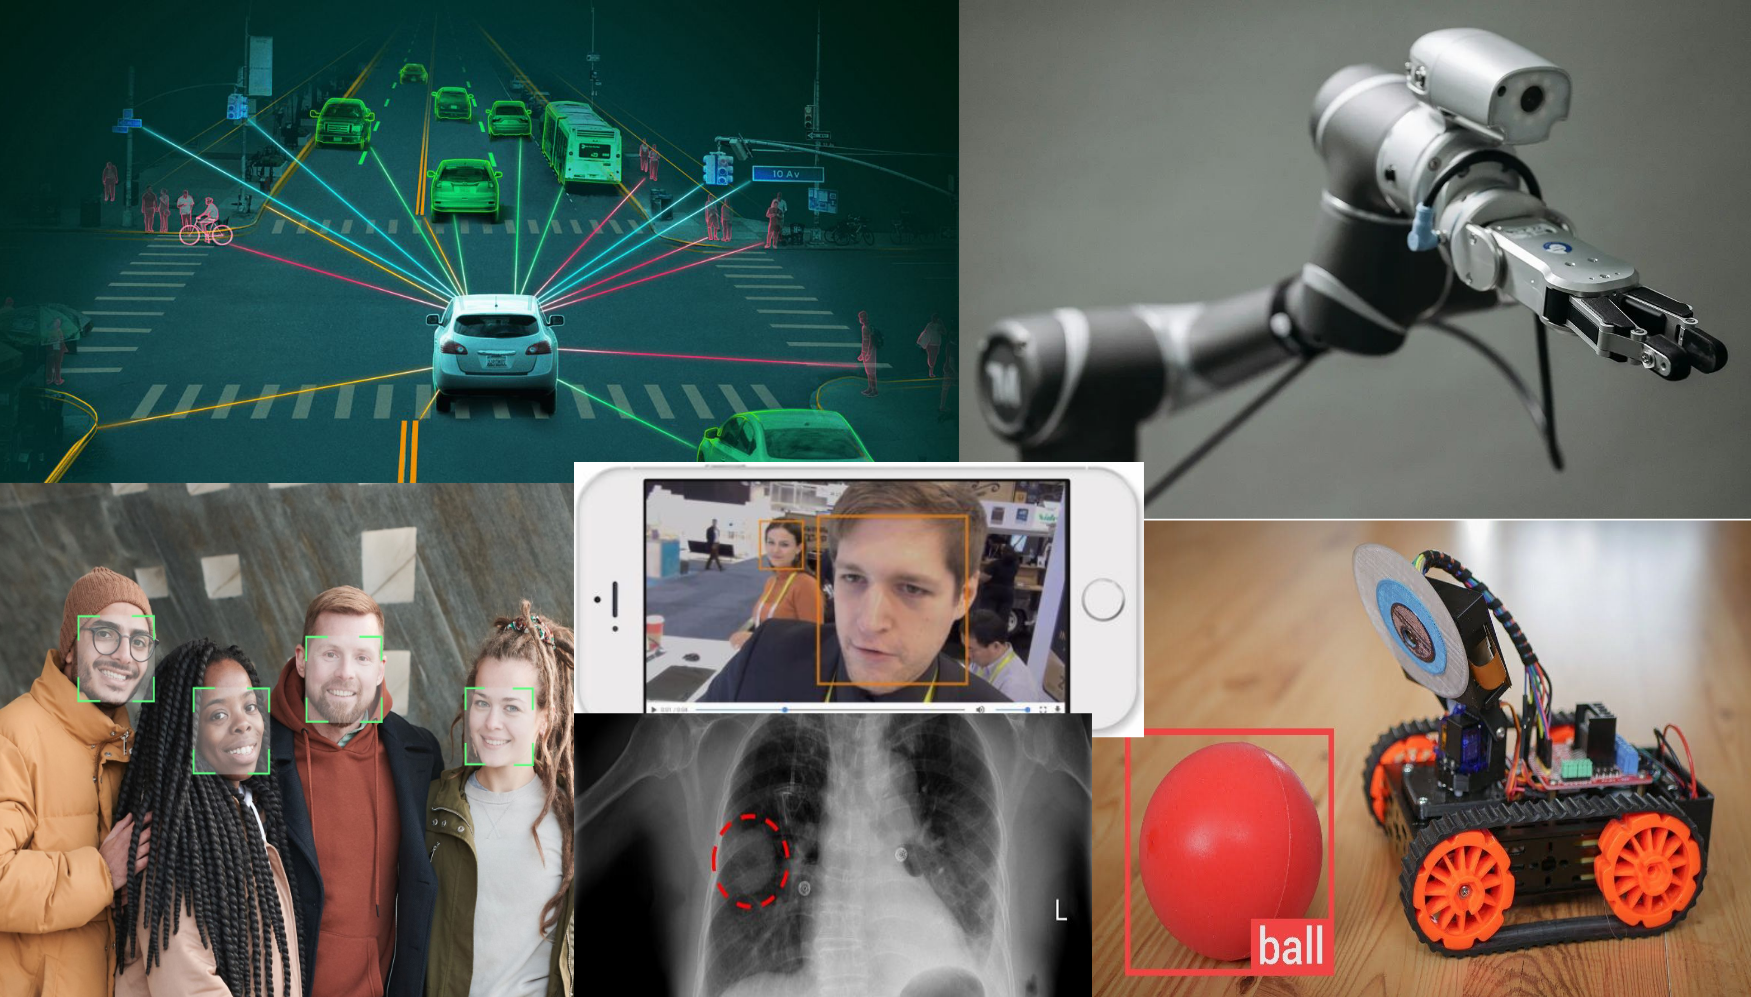
\includegraphics[width=\linewidth]{Pictures/CNN_1.png}
    \end{subfigure}
\end{figure}

\subsection{Why do MLPs struggle on images?}
\subsubsection{Spatial adjacency}
In an image, pixels that are adjacent are strongly correlated and form meaningful patterns like edges, corners, and textures. 
When a 2D image is flattened into a 1D array, vertical neighbors are separated across the vector. 
Standard dense layers treat all input elements identically without encoding geometric or spatial structure.
\subsubsection{Parameter explosion}
In a dense layer, every input unit connects to every hidden neuron. For a color image of size $1000\times 1000\times 3$, the input vector has 3000000 dimensions.
Connecting this to a single hidden layer of just 1000 neurons would require $3\times 10^6\times 10^3=3$ billion weights (plus biases).
This computational burden causes expensive memory usage, high latency, and severe overfitting.
\subsubsection{Inability to handle visual variations}
A standard MLP must re-learn the pattern separately at every single pixel position because it lacks translation invariance.
Real-world computer vision must remain invariant to seven fundamental visual challenges:
\begin{enumerate}
    \item \textbf{Intra-class variance:} In other words, each class needs diverse shapes, sizes, colors, etc. 
    \item \textbf{Transformation variance:} Non-rigid transformations. For example, take a dog. When a dog is curled up or lying down, we still need to be able to classify it as a dog.
    \item \textbf{Viewpoint variance:} Viewing an object from various perspectives and angles.
    \item \textbf{Scale variance:} Viewing an object appearing very large (close to the camera) or very small (far away from the camera).
    \item \textbf{Illumination variance:} Shifts in lighting, shadows, and contrast.
    \item \textbf{Occlusion:} Objects partially hidden behind other objects/entities, i.e. a leopard hiding behind a rock.
    \item \textbf{Background clutter:} Objects blending into complex environments (camouflage).
\end{enumerate}

\subsection{CNN architecture}
\subsubsection{Local receptive fields}
Instead of connecting a hidden neuron to every pixel in the image, each neuron connects only to a small, localized sub-region of the input.
This perserves the adjacency of the pixels. This also reduces the weight count significantly. If each region covers $k$ pixels ($k\ll n$), the number of connections per node drops from $n$ to $k$.
\subsubsection{The convolution operation}
A \textbf{kernel} (or \textbf{filter}) is a small learnable weight matrix, typically $2\times 2$. 
The kernel slides systematically across the input image patch-by-patch. A each location, the network computes an element-wise multiplication between the kernel weights and current image patch, then sums the products (a dot product) to produce a signle value in the feature map.
\subsubsection{Multiple kernels per layer}
A single filter can only detect one specific feature type. To capture varied visual patterns, each layer uses multiple independent filters.
convolving a $6\times 6$ image with two separate $3\times 3$ filters produces two $4\times 4$ feature maps, resulting in an output volume of dimension $4\times 4\times 2$.
\subsubsection{Feature detection}
Although each individual filter remains small (e.g. $3\times 3$), stacking layers allows a neuron in a deeper layer to span a wider area of the original input, giving it a broader context window.
\begin{itemize}
    \item \textbf{Layer 1:} Detects basic visual stimuli such as oriented edges, color transitions, and lines.
    \item \textbf{Layer 2:} Combines edge primitives to detect corners, textures, curves, etc.
    \item \textbf{Layer 3+:} Combines mid-level shapes to recognize complex structural parts and whole objects.
\end{itemize}

\subsection{Convolution operation}
\subsubsection{2D cross-correlation}
For a 2D matrix $I$ and a $k\times k$ kernel $K$, the activation at output coordinate $(i,j)$ is defined as:
$$
S(i,j)=(K\ast I)(i,j)=\sum_m\sum_nI(i+m,j+n)K(m,n)
$$
\textbf{Example:}
\begin{align*}
\underbrace{\begin{bmatrix}
1 & 2 & 3 & 4 \\
5 & 6 & 7 & 8 \\
9 & 10 & 11 & 12 \\
13 & 14 & 15 & 16
\end{bmatrix}}_I
\ast
\underbrace{\begin{bmatrix}
0 & -1 & 0 \\
-1 & 5 & -1 \\
0 & -1 & 0
\end{bmatrix}}_K
+\underbrace{5}_b
=\begin{bmatrix}
11 & 12 \\
15 & 16
\end{bmatrix}
\end{align*}
\subsubsection{Multi-channel 3D convolutions}
Color images contain multiple channels, e.g. RGB has 3 channels. A kernel in a multi-channel layer must match the exact depth of the input volume.
For an input with $C$ channels, a $k\times k$ filter has spatial dimensions $k\times k\times C$. 
The filter performans a 2D convolution over each channel independently. The resulting scalar values across all channels are then summed together with the bias to produce one single 2D feature map slice.
$$
\text{Output}(i,j)=\Large\Big(\sum_{c=1}^C\sum_m\sum_nI_c(i+m,j+n)K_c(m,n)\Big)
$$
\subsubsection{Using multiple filters per layer}
Because a single filter can only extract one specific feature type, a layer uses $d$ distinct filters.
Each filter produces its own 2D feature map. Stacking the output yields a feature volume of depth $d$.
For $d$ filters of size $k\times k$ over an input with $c$ channels:
$$
\text{Total Learnable Parameters}=d\times(k^2\cdot c+1)\quad \text{(Including 1 bias per filter)}
$$
Notice that the number of parameters is completely independent of the input image's size.

\subsection{Calculating the output size}
The dimensions of a feature map depend on four parameters:
\begin{enumerate}
    \item Input size (width and height)
    \item Filter size
    \item Padding
    \begin{itemize}
        \item Without padding, the filters cannot extend past the edges, which progressively shrinks the output map.
    \end{itemize}
    \item Stride
    \begin{itemize}
        \item The step size by which the filter slides across the image.
    \end{itemize}
\end{enumerate}
For an input of size $W\times H$, filter size $K\times K$, symmetric padding $P$, and stride $S$:
$$
W_{\text{out}}=\Big\lfloor\frac{W-K+2P}{S}\Big\rfloor+1 \quad\quad
H_{\text{out}}=\Big\lfloor\frac{H-K+2P}{S}\Big\rfloor+1
$$
Then, the output shape is $(W_{\text{out}},H_{\text{out}},d)$ for $d$ distinct filters.
\\\\
\textbf{Example:}\\
Suppose we are training on $256\times 256$ RGB images with a batch size of 64. The input is a 4-dimensional tensor of size $256\times 256\times 3\times 64$.
Now apply 96 kernels of size $5\times 5\times 3$ with a stride of 2 in both directions.
$$
W_{\text{out}}=\Big\lfloor\frac{256-5+2(2)}{2}\Big\rfloor+1=128 \quad\quad
H_{\text{out}}=\Big\lfloor\frac{256-5+2(2)}{2}\Big\rfloor+1=128
$$
Then, the output tensor is of size $128\times 128\times 96\times 64$ ($W_{\text{out}}\times H_{\text{out}}\times \text{Channels}\times \text{Batch Size}$).
\subsection{3D convolution as matrix multiplication}
\textbf{Example 1:}\\
Given $d=64$ filters, each of shape $c\times k\times k=3\times 3\times 3$ and an input image with size $32\times 32$, flatten each 3D filter into a row vector of length $3\times 3\times 3=27$.
$$
\text{Weight Matrix Shape}=d\times (c\cdot k^2)=64\times 27
$$
Extract every local $3\times 3\times 3$ receptive field patch from the input ($3\times 32\times 32$) and flatten each patch into a column vector of length 27.
For an output grid of $32\times 32=1024$ patch positions, align these column side-by-side:
$$
\text{Feature Matrix Shape}=(c\cdot k^2)\times(w\cdot h)=27\times 1024
$$
Computing the standard 2D matrix dot product:
$$
Y_{\text{mat}}=(64\times 27)\times(27\times 1024)=64\times 1024
$$
Reshape the resulting $64\times 1024$ matrix back into the target 3D tensor: $64\times 32\times 32$.

\subsection{Non-linearity and pooling}
Every convolution block combines linear filtering with non-linear activation and downsampling.
\subsubsection{Non-linearity}
CNNs apply an element-wise activation function, typically ReLU, directly after a convolution.
ReLU introduces non-linear decision boundaries while perserving gradient flow during backpropagation.
\subsubsection{Pooling (downsampling)}
Pooling reduces the spatial size of the feature map using a fixed aggregation function over sliding windows.
Unlike convolutional kernels, pooling filters do not have weights or biases. Their operation is fixed.
It serves two purposes:
\begin{enumerate}
    \item \textbf{Computational efficiency:} Downsamples spatial dimentionality, reducing the memory footprint and the number of parameters required in downstream layers.
    \item \textbf{Translational invariance:} Summarizing local windows makes the model robust to small shifts in feature locations.
\end{enumerate}
\textbf{Max pooling vs. Average Pooling}\\
Both operations slide a window of size $l\times l$ with stride $s$.
\\\\
\begin{tblr}{width=\textwidth, colspec={l X[l] X[l]}, row{1}={font=\bfseries}}
\toprule
Feature & Max Pooling & Average Pooling \\
\midrule
Operation & Selects $\max\{x_1,x_2,\dots,x_n\}$ in the window. & Computes $\frac{1}{n}\sum_{i=1}^n x_i$ over the window. \\
Visual role & Acts like a boolean \textbf{OR gate}. It records whether a feature appeared anywhere in the window. & Smooths activations. It retains background context. \\
\bottomrule
\end{tblr}
\begin{figure}[H]
    \centering
    \begin{subfigure}{0.8\textwidth}
        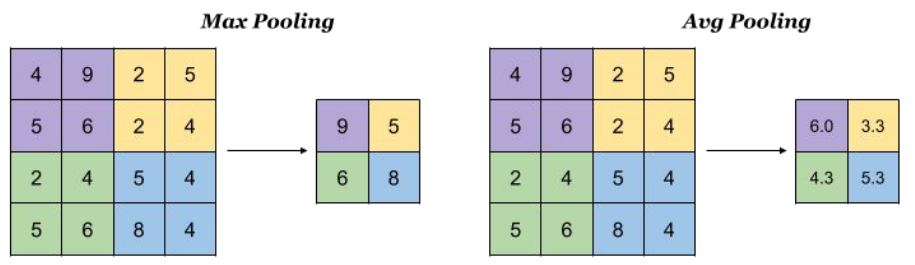
\includegraphics[width=\linewidth]{Pictures/CNN_2.png}
    \end{subfigure}
\end{figure}

\subsection{Convolutional layer vs. pooling layer}
The convolutional layer and pooling layer server distinct mathematical and functional roles in the network:
\\\\
\begin{tblr}{width=\textwidth, colspec={l X[l] X[l]}, row{1}={font=\bfseries}}
\toprule
Property & Convolutional layer & Pooling layer \\
\midrule
Primary objective & Feature extraction and localized pattern detection. & Spatial downsampling and feature aggregation. \\
Learnable parameters & Contains learnable weights $K$ and biases $b$ updated via backpropagation. & Zero learnable parameters. It applies fixed deterministic functions. \\
Invariance & Translation equivariant & Translation invariant \\
\bottomrule
\end{tblr}

\subsection{Macro architecture}
\begin{figure}[H]
    \centering
    \begin{subfigure}{0.8\textwidth}
        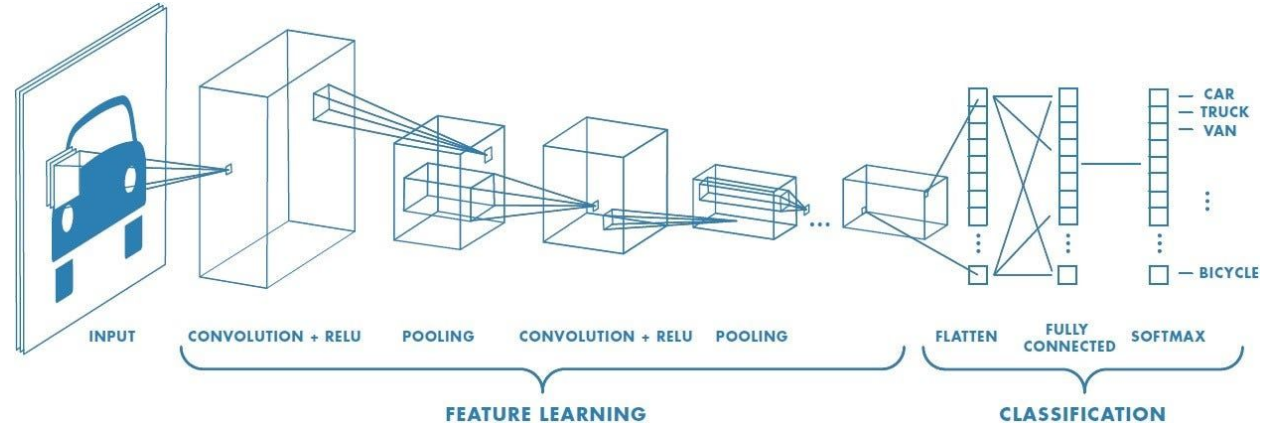
\includegraphics[width=\linewidth]{Pictures/CNN_3.png}
    \end{subfigure}
\end{figure}
A full CNN is divided into two distinct components: the feature extractor and the classifier.
\begin{itemize}
    \item \textbf{The feature extractor:} Transforms raw pixel values into abstract, high-level semantic feature representations using stacked [Conv$\to$ReLU$\to$Pool] blocks. As representations move deeper, spatial dimensions contract while feature depth expands.
    \item \textbf{The bridge (flattening):} A parameter-free reshape layer that converts the 3D tensor output of the final pooling layer ($W\times H\times C$) into a flat 1D feature vector of length $W\cdot H\cdot C$.
    \item \textbf{The classifier head (dense MLP):} Standard fully connected layers that take the global feature vector, model non-linear interactions across all extracted features, and project them to class logits before computing normalized probabilities via softmax.
\end{itemize}

\subsection{Backpropagation in CNNs}
\subsubsection{Backpropagation through convolutional layers}
The backward pass through a convolutional layer is itself a convolutional operation. Let the layer's forward pass be $Y=X\ast K$, where $\frac{\partial \mathcal{L}}{\partial Y}$ is the upstream error gradient received from the subsequent layer.
\\\\
\textbf{Gradient w.r.t filer weights ($\frac{\partial \mathcal{L}}{\partial K}$):}\\
The gradient of the loss with respect to the kernel weights $K(m,n)$ is the convolution between the input $X$ and the upstream output gradient $\frac{\partial \mathcal{L}}{\partial Y}$:
$$
\frac{\partial \mathcal{L}}{\partial K}=X\ast\frac{\partial \mathcal{L}}{\partial Y}
$$
\\\\
\textbf{Gradient w.r.t layer inputs ($\frac{\partial \mathcal{L}}{\partial X}$):}\\
To pass the gradient back to the preceding layer, the upstream gradient $\frac{\partial \mathcal{L}}{\partial Y}$ is convolved with the spatially rotated (flipped by 180$^{\circ}$) kernel $K^{\text{rot}}$:
$$
\frac{\partial \mathcal{L}}{\partial X}=\frac{\partial \mathcal{L}}{\partial Y}\ast K^{\text{rot}}
$$
\\\\
\textbf{Gradient w.r.t biases ($\frac{\partial \mathcal{L}}{\partial b}$):}\\
Because a single scalar bias $b$ is shared across the entire spatial feature map, its gradient is the sum of all elements in the upstream error map:
$$
\frac{\partial \mathcal{L}}{\partial b}=\sum_i\sum_j\Big(\frac{\partial \mathcal{L}}{\partial Y}\Big)_{i,j}
$$
\subsubsection{Backpropagation through max pooling layers}
Because max pooling contains no weights, it does not generate parameter updates. However, it must route upstream error gradients back to the preceding layer.
There is a routing problem. Max pooling discards 75\% of activation values (in a $2\times 2$ window) during the forward pass. Non-maximal neurons have a local forward derivative of zero ($\frac{\partial y}{\partial x_i}=0$), so they do not receive gradient signals.
A solution to this problem is the \textbf{winner-takes-all mechanism}. The network stores the coordinate of the maximum value within each pooling window:
$$
\text{Mask}(i,j)=\begin{cases}
    1 & \text{if }x_{i,j}=\max(\text{Window}) \\
    0 & \text{otherwise}
\end{cases}
$$
The upstream gradient $\frac{\partial \mathcal{L}}{\partial Y}$ is passed exclusively to the winning neuron, while all non-maximal neurons receive a gradient of 0:
$$
\frac{\partial \mathcal{L}}{\partial X_{i,j}}=\frac{\partial \mathcal{L}}{\partial Y}\cdot\text{Mask}(i,j)
$$

\section{Unsupervised Learning}
\subsection{What is unsupervised learning?}
The unsupervised learning problem is framed as finding structure in $x$ without labels $y$. Inputs are examples in the dataset represented by features.
Given a new example $x$ where does this fit into the data? We start with a dataset that does not contain labels and seek to discover interesting and useful patterns in this data, such as:
\begin{itemize}
    \item \textbf{Clusters:} Find clusters of related data points across the dataset. For example, groups of similar e-commerce customers.
    \item \textbf{Dimensionality:} Identify features that explain the most important parts of the data (dimensionality reduction). For example, SKA data compression.
    \item \textbf{Missing values:} Predict missing values based on similar entries in the data. For example, user movie rating prediction.
    \item \textbf{Detect outliers:} Detect outliers, i.e. particularly unusual or interesting data points. For example, suspicious financial transactions.
\end{itemize}

\subsection{Outlier detection}
\begin{figure}[H]
    \centering
    \begin{subfigure}{0.5\textwidth}
        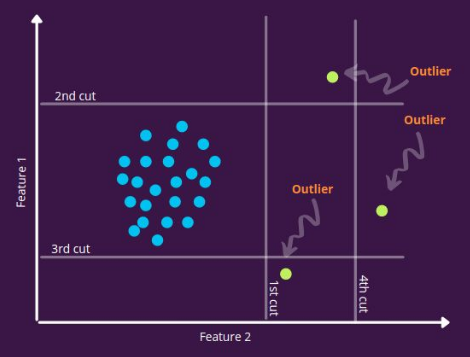
\includegraphics[width=\linewidth]{Pictures/CNN_5.png}
    \end{subfigure}
\end{figure}

\subsection{Dimensionality reduction}
For example, principal component analysis (PCA).
\begin{figure}[H]
    \centering
    \begin{subfigure}{0.6\textwidth}
        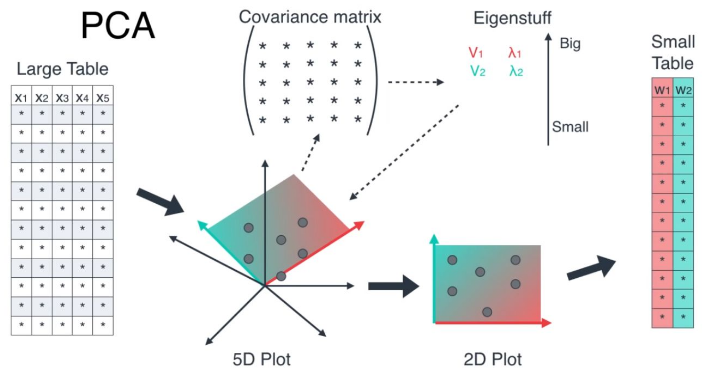
\includegraphics[width=\linewidth]{Pictures/CNN_6.png}
    \end{subfigure}
\end{figure}
$\quad$\\[-1em]
Some use cases:
\begin{itemize}
    \item \textbf{Visualization} of high-dimensional in 2D or 3D (e.g. using t-SNE).
    \item \textbf{Compression} of large datasets.
    \item \textbf{Reduce computational cost} for data processing or as input to other machine learning models.
\end{itemize}

\subsection{Clustering}
\begin{figure}[H]
    \centering
    \begin{subfigure}{0.5\textwidth}
        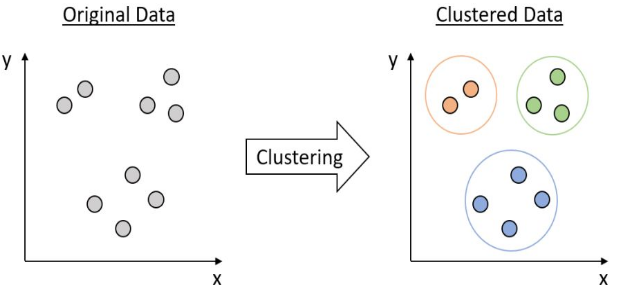
\includegraphics[width=\linewidth]{Pictures/CNN_4.png}
    \end{subfigure}
\end{figure}
$\quad$\\[-1em]
We group data into potentially useful groups. This is perhaps the most common unsupervised learning task.
\begin{itemize}
    \item Automatically organize data and simplify data for further analysis.
    \item Can lead to a better understanding of data.
    \item Dsicovering groups of data can have practical value.
\end{itemize}
Here are some key practical uses:
\begin{itemize}
    \item \textbf{Recommendation systems:} Group similar items/users together and make movie recommendations based on these clusters.
    \item \textbf{Anomaly detection:} Points that do not belong to any cluster (outliers) or are far from other clusters can be flagged as anomalies.
    \item \textbf{Image segmentation:} Divide images into regions based on pixel similarity. Useful in applications such as object recognition.
    \item \textbf{Document clustering:} Clustering groups similar documents together. useful for topic modeling and information retrieval.
\end{itemize}
What properties should good clustering of a dataset have?
\begin{itemize}
    \item Data points inside each cluster are close together $\Rightarrow$ \textbf{Intra-cluster} similarity is minimized.
    \item Data points in different clusters are far apart $\Rightarrow$ \textbf{Inter-cluster} similarity maximized.
\end{itemize}
\subsubsection{Two types of clustering algorithms}
\textbf{Hierarchical clustering:}\\
Clusters form a nested hierarchy. Agglomerative (bottom-up) starts with samples and merges samples in groups according to some criteria. Divisive (top-down) splits the data into clusters.
\\\\
\textbf{Partitional/Flat clustering:}\\
No inter-cluster structure. Flat partitioning directly partitions data into distinct, non-overlapping subsets without building parent-child relationships between clusters.
\begin{figure}[H]
    \centering
    \begin{subfigure}{0.6\textwidth}
        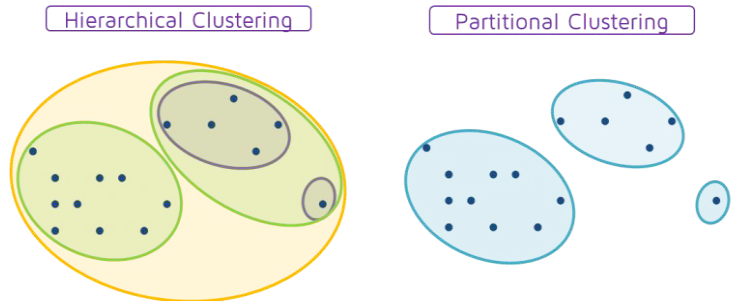
\includegraphics[width=\linewidth]{Pictures/CNN_7.png}
    \end{subfigure}
\end{figure}
\subsubsection{Decisions for clustering}
There are two options for the distance function:
\begin{enumerate}
    \item \textbf{Euclidean distance}
    $$
    d(p,q)=||q-p||=\sqrt{\sum_{i=1}^{n}(q_i-p_i)^2}
    $$
    \item \textbf{Cosine similarity}
    $$
    d(p,q)=\frac{p\cdot q}{||p||\cdot||q||}
    $$
\end{enumerate}
Which clustering algorithm? \textbf{K-means clustering}.
\begin{figure}[H]
    \centering
    \begin{subfigure}{0.6\textwidth}
        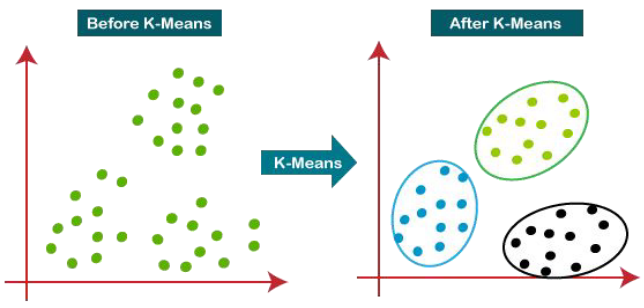
\includegraphics[width=\linewidth]{Pictures/CNN_8.png}
    \end{subfigure}
\end{figure}
\end{document}